\documentclass[notitlepage, superscriptaddress]{revtex4-2}
% \documentclass[aps, prl, preprint, superscriptaddress, longbibliography]{revtex4-1}
%%%%%%%%%%%%%%%%%%%%%%%%%%%%%%%%%%%%%%%%%%%%%%%%%%%%%%%%%%%%%%%%%%%%%
\usepackage{amsmath}
\usepackage{hyperref}
\usepackage{latexsym}
\usepackage{graphicx}
\usepackage[usenames,dvipsnames]{xcolor}
\usepackage{bm}
\usepackage[normalem]{ulem}
\usepackage{bbold}
\setcounter{MaxMatrixCols}{60}


\begin{document}

\title{SEIR-C: An epidemic model that includes contact tracing}

\author{Lynden K. Shalm}
% \affiliation{Associate of the National Institute of Standards and Technology, Boulder, Colorado 80305, USA}
\affiliation{Department of Physics, University of Colorado, Boulder, Colorado, USA}
\author{Jasper Palfree}
% \affiliation{Associate of the National Institute of Standards and Technology, Boulder, Colorado 80305, USA}
\affiliation{Department of Physics, University of Colorado, Boulder, Colorado, USA}

% \author{Sae Woo Nam}
% \affiliation{National Institute of Standards and Technology, 325 Broadway, Boulder, CO 80305, USA}

\begin{abstract}
The SEIR model has been widely used to study the dynamics of pandemics. Here we update the model to include the effects of contact tracing as a means to control the outbreak. We call this new model SEIR-C.
\end{abstract}
\date{\today}
\maketitle

%%%%%%%%%%%%%%%%%%%%%%%%%%%%%%%%%%%%
\section{Introduction to SEIR}
%%%%%%%%%%%%%%%%%%%%%%%%%%%%%%%%%%%%

The SEIR model relies on a set of differential equations to model the transmission dynamics of an infectious disease. A susceptible population ($S$) has some probability of coming into contact with the infected population ($I$) while they still infectious for some time ($\tau_{inf}$). Those from $S$ who have contracted the disease are then classified as having been exposed ($E$). Those who are exposed are not infectious, but rather the disease takes some time ($\tau_{inc}$) to incubate, after which point they move to the infectious population. Individuals who are in $I$ will eventually recover after a time $\tau_{inf}$. At this point they are assumed to have achieved immunity or have died. For the situation considered here, we also assume that birth rates and death rates are equal so the total population remains constant. Therefore, the total population $N$ is given by:
\begin{eqnarray}
\label{E:SEIRPop}
N = S + E + I + R.
\end{eqnarray}

In the standard SEIR model the rate of change for each of the different disease stages are given as a set of coupled differential equations:
\begin{eqnarray}
\label{E:SEIR}
\frac{dS}{dt} &=& - \beta_0 \frac{I}{N}S, \\
\frac{dE}{dt} &=& \beta_0 \frac{I}{N}S - \frac{1}{\tau_{inc}}E, \\ 
\frac{dI}{dt} &=& \frac{1}{\tau_{inc}}E - \frac{1}{\tau_{inf}}I, \\ 
\frac{dR}{dt} &=& \frac{1}{\tau_{inf}}I.
\end{eqnarray}

Here $\beta_0 = \frac{R_{0}}{\tau_{inf}}$, where $R_{0}$ is the average number of people an infectious person in $I$ will infect and is known as the reproduction number. The rate at which the exposed population increases is therefore related to how fast an infectious person spreads the disease ($\beta_{0}$) times the fraction of the population that is infectious ($I/N$) multiplied by the number of people who are susceptible ($S$).

A modified SEIR model that is widely used also accounts for asymptomatic individuals, and can track hospitalizations and deaths. We will use this version of SEIR as our starting point, and then add in testing and contact tracing in a way that allows their effects to be studied somewhat independently (contact tracing is heavily dependent on testing, but it is possible to study the effects of testing independent of contact tracing). The modified model is shown if figure \ref{f:simpleSEIR}.

\begin{figure}
\centering
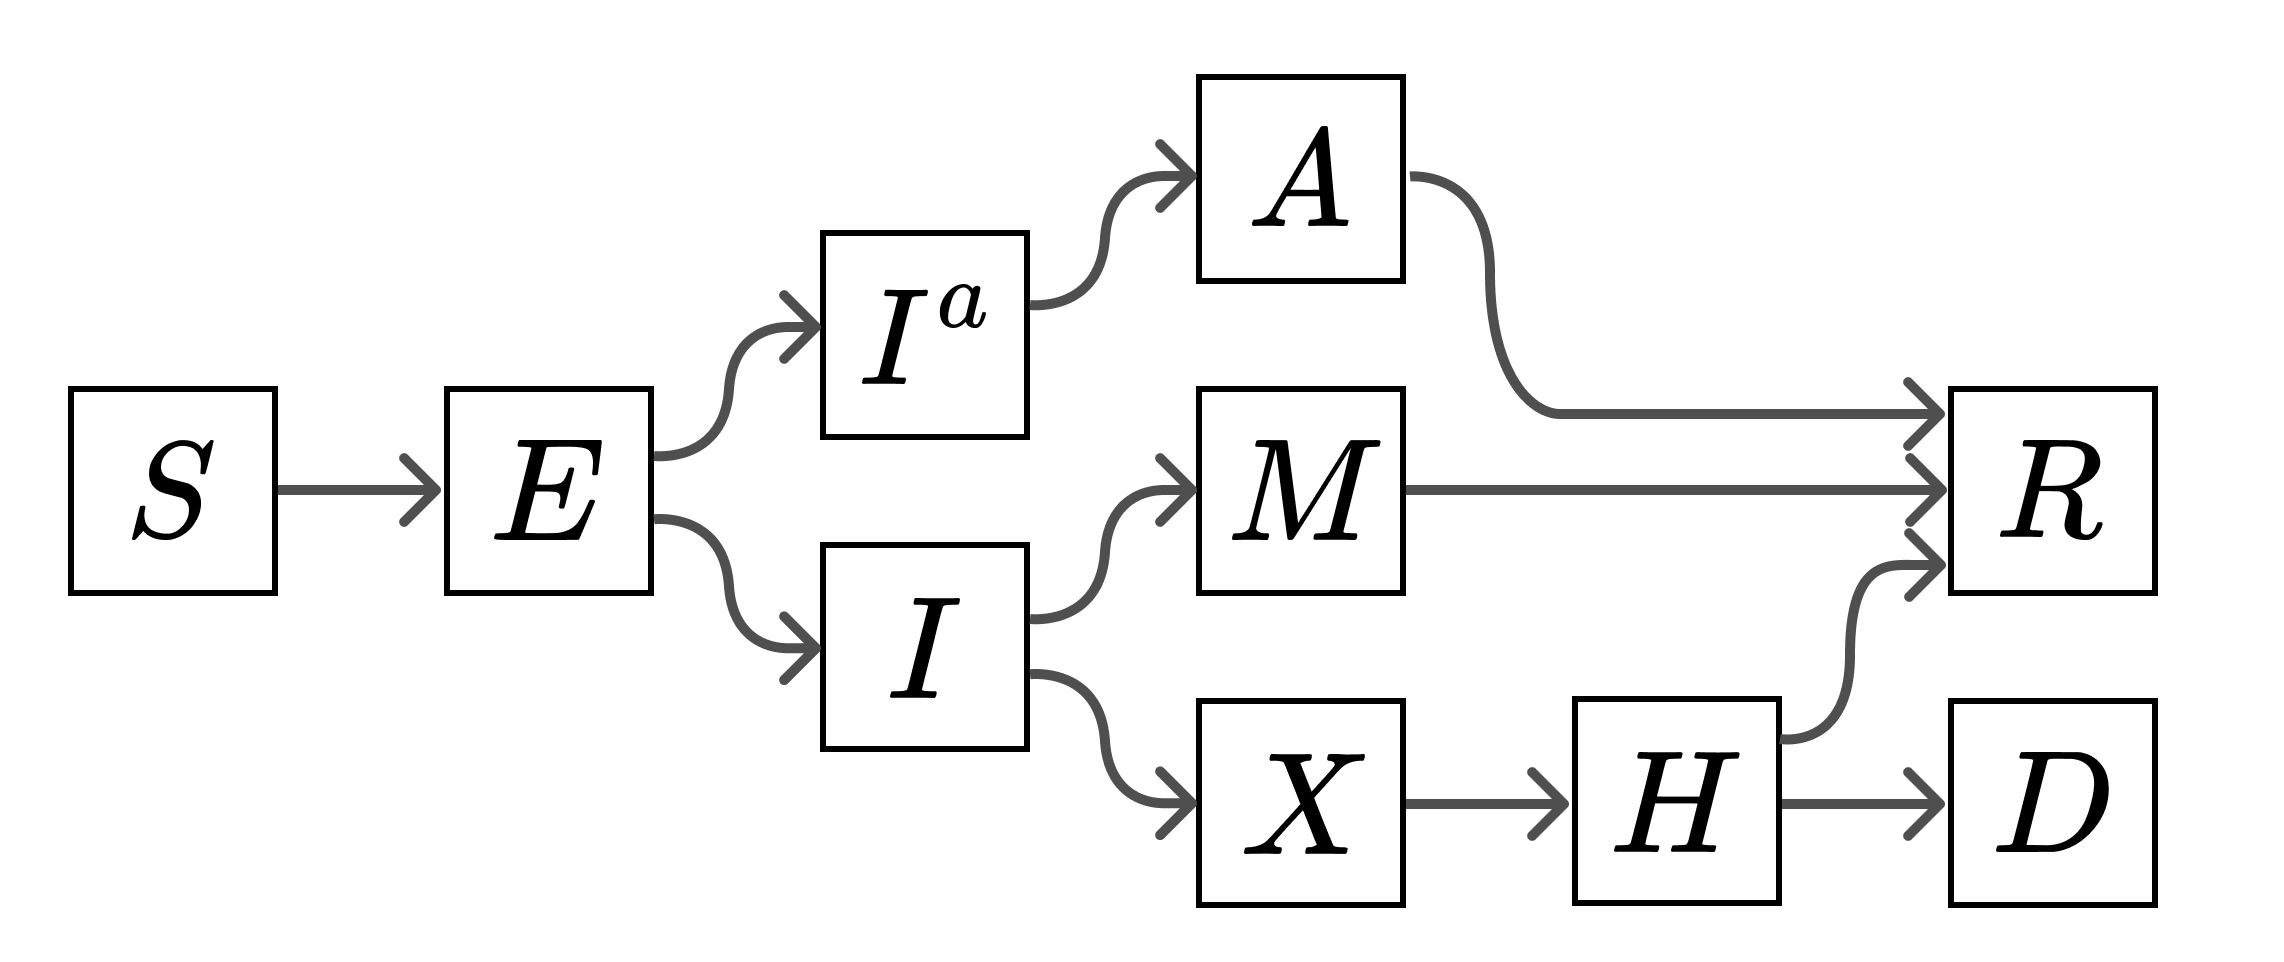
\includegraphics[width=5in]{Basic_SEIR}
\caption{\label{f:simpleSEIR}
 Conceptual diagram for SEIR with asymptomatic individuals. The first population group are those who are susceptible ($S$), meaning they have not yet been infected. They can become infected through contact with someone who is infectious ($I$ and $I^{a}$). Once infected, they move to the exposed group ($E$) for some incubation period $\tau_{inc}$. During this time they cannot infect others. Next, they move to the infectious phase of the disease for an average time $\tau_{inf}$ where it can be spread to others through contact. There are two infectous populations, those who show symptoms ($I$), and those who are asymptomatic ($I^{a}$). Once the infectious phase is finished, those who are asymptomatic move to the population $A$ where they are still sick but no longer infectious. After a time $\tau_{a}$ they recover ($R$), meaning they have developed immunity and can not be reinfected. Those who show symptoms will either progress to to the mild population ($M$) where they will eventually recover after an average time $\tau_{mild}$, or they will develop severe symptoms ($X$) that will eventually require hospitalization ($H$) after an average time $\tau_{h}$. Those who are hospitalized will either recover after an average time $\tau_{sev}$, or die ($D$) after an average time $\tau_{d}$.}
\end{figure}


%%%%%%%%%%%%%%%%%%%%%%%%%%%%%%%%%%%%
\section{SEIR with testing (SEIR-T)}
%%%%%%%%%%%%%%%%%%%%%%%%%%%%%%%%%%%%
We will first extend the basic SEIR model described in the previous section to include testing. An important consideration is how long it takes to get test results on average ($\tau_{t}$), as well as the percentage of tests that return a false positive ($f_{pos}$) or a false negative $f_{neg}$. In general, the probability that someone will be given a test is $p_{t}$, but it is possible to test those who show symptoms ($p^{i}_t$) as well as those who are hospitalized ($p^{sev}_{t}$) at a higher rate. 

For each of the different populations $S$, $E$, $I$, $I^{a}$, $A$, $M$, $X$, and $H$, we consider three different subpopulations. There are those who have not yet been tested (which we denote with a ``$g$'' subscript, i.e. $S_{g}$), those who have been tested but are waiting for their results (denoted by a ``$w$'', i.e. $S_{w}$), and finally those who have tested positive (denoted a ``t'' subscript, i.e. $S_{t}$). In figure XXX each of these not tested, waiting, and positive tests are represented as layers. To simplify matters, individuals can move between layers within their current population group, but when transitioning to a the next phase of the disease must stay within their layer. For example, someone who is in the exposed phase and waiting for their test results, $E_{w}$ can move to $E_{t}$ if they test positive. They also have a chance of moving to the infectious phase $I_{w}$ where they continue to wait for their test results. However, they cannot move to $I_{t}$ directly from $E_{w}$ ($E_{w} \rightarrow I_{t}$). Instead they have to follow the path $E_{w} \rightarrow I_{w} \rightarrow I_{t}$.  

We assume that those who are waiting for their test results quarantine themselves. If an individual tests positive, then they continue to quarantine for an average time of $\tau_{iso}$, after which they return to the general population. We assume that anyone who has tested positive will not be tested again unless their quarantine period ends before recovery and they return to the non-tested population. Those who develop severe symptoms and are hospitalized will remain quarantined. For those in the susceptible population who are quarantined, this leads to a reduction in their probability of infection by a factor $d_{r}$. For those in the infectous group who are quarantining, their ability to infect others ($R_{0}$) is reduced by a factor $d_{r}$. If an individual tests negative while in $S_{w}$ they return to $S_{g}$ and stop quarantining. Similarily, those who are infectious that test negative (through a false negative) will return to either $I_{g}$ or $I^{a}_{g}$ where they will resume infecting others at the original $R_{0}$.  

\begin{figure}
\centering
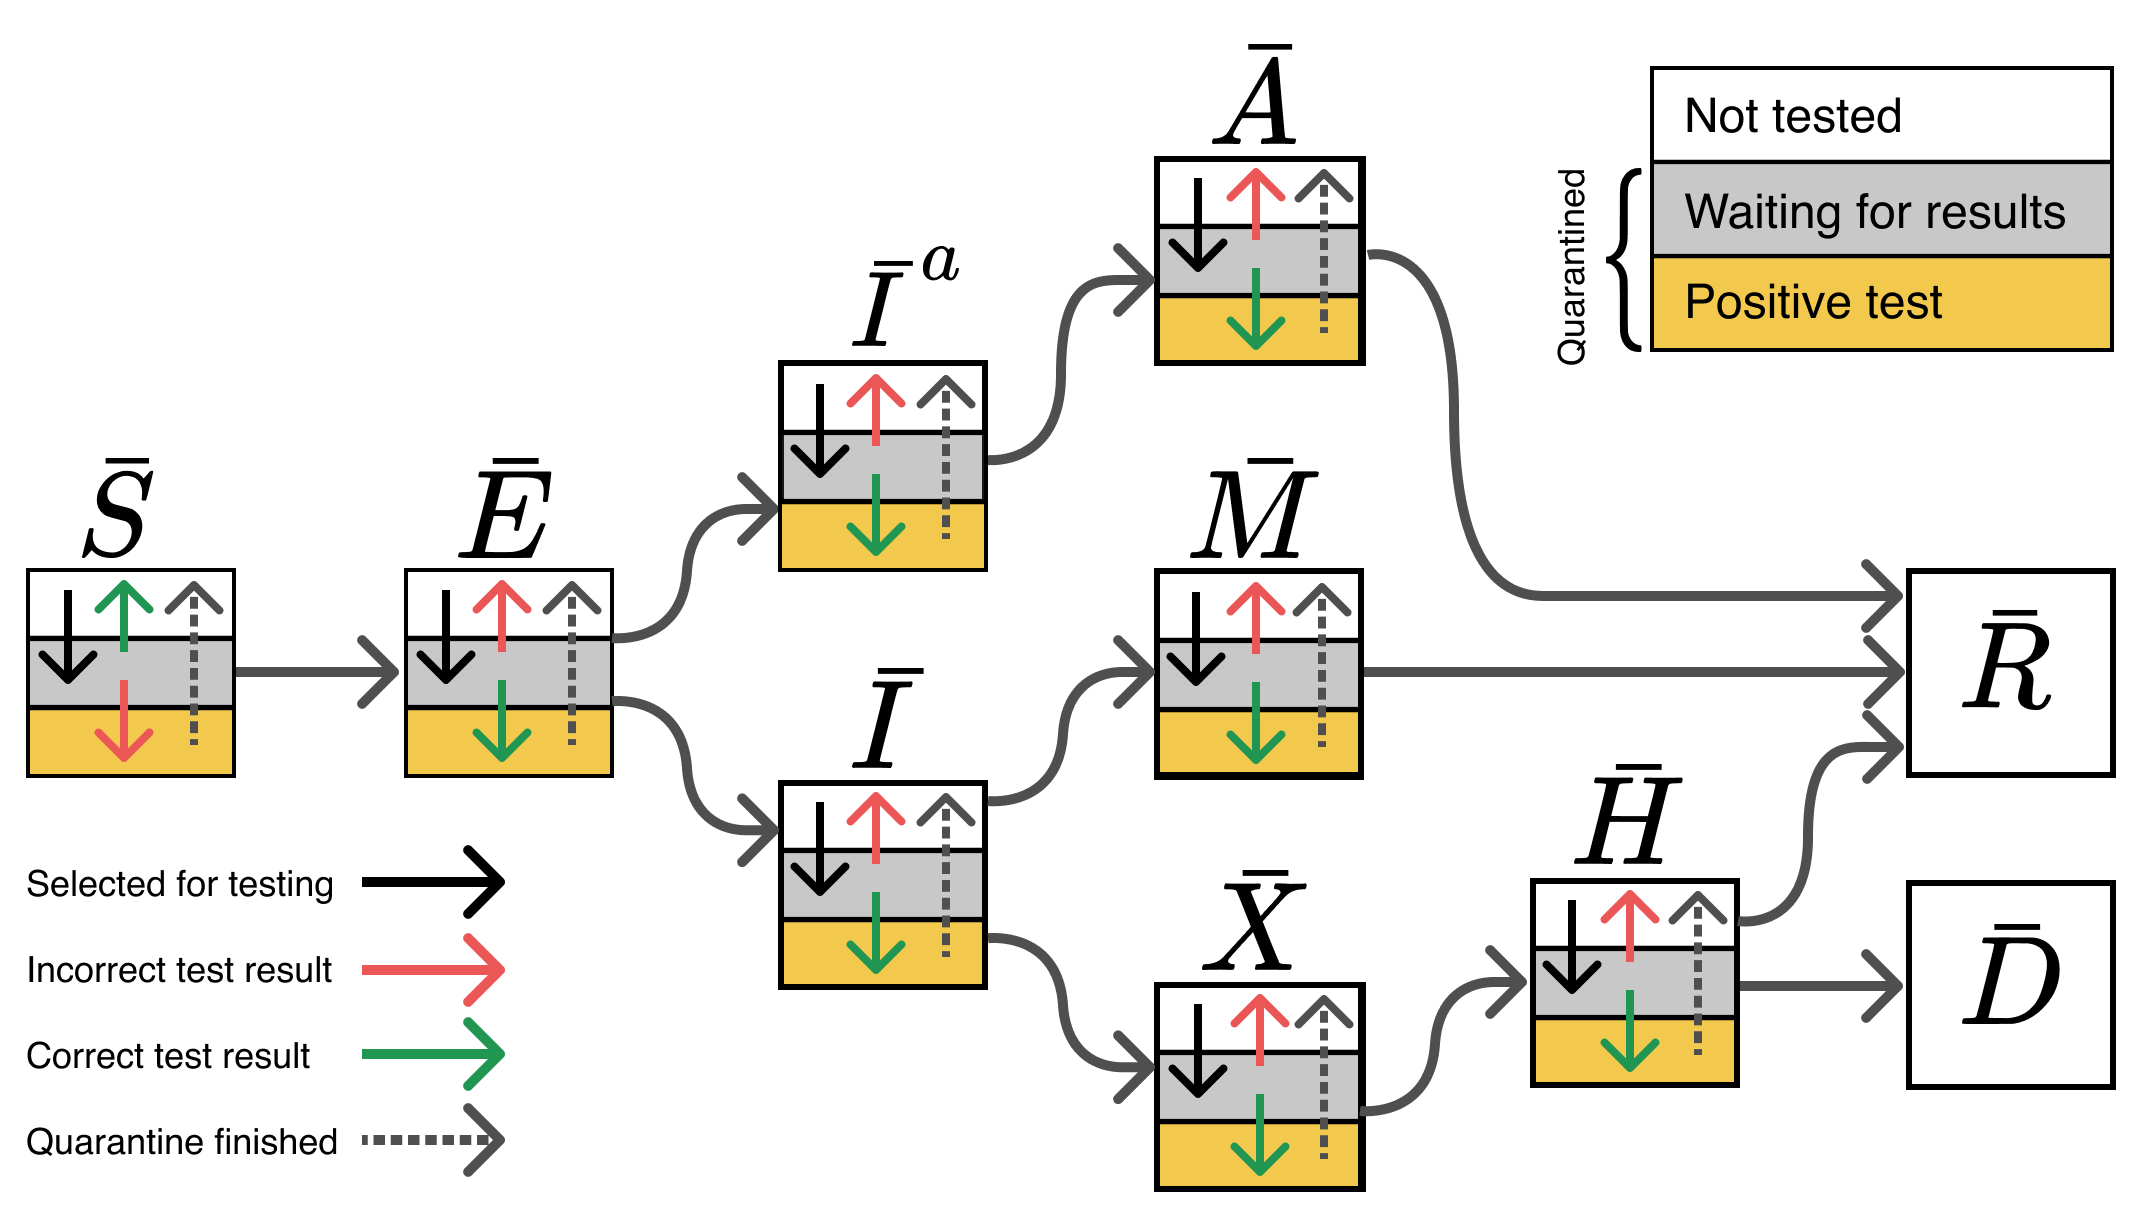
\includegraphics[width=5in]{SEIR_testing_no_contact}
\caption{\label{f:SEIR-testing}
SEIR with testing incorporated. It is convenient to divide each population into three subgroups, those who have not been tested (white), those who have been tested but are waiting for their results (grey), and those who have tested positive (yellow). Anyone in the white or yellow layers is quarantined. When transitioning between disease phases, individuals can only move to the same color layer (for example $E_{w} \rightarrow I_{w}$ or $I_{g} \rightarrow M_{g}$). Vertical arrows represent the transitions that can occur within a population group. Black arrows represent movement due to testing, red arrows represent movement due to an incorrect test result (false positive for those in susceptible, false negative for all other populations), green arrows show movement due to a correct test result, and the dashed arrow show individuals who have finished their quarantine period.}
\end{figure}


\section{SEIR with contact tracing (SEIR-C)}
We can further build on the SEIR model with testing to incorporate contact tracing. @TODO define contact tracing and what we consider. 

The model assumes that a fraction of the population $p_{c}$ chooses to particpate in contact tracing. We therefore divide the population in those who do not contact trace and those that do, and treat their population dynamics separately. Someone who starts in the contact tracing group cannot migrate to the non contact tracing population, but someone who is contact tracing can infect someone who is not (and vice-versa). As shown in figure XXXX, we now have two separate sets of population transfer dynamics to consider. We label all the population groups who do not participate in contact tracing with a bar accent (for example, $\bar{S}$), and those who do particpate with a check accent (for example, $\check{E}$). We keep this notation throughout. 

The flow of the population not particpating in contact tracing reduces to the case where we only have testing (as shown in figure XXXXX). However, those particpating in contact tracing have additional states that need to be considered as shown in figure XXXXX.

\begin{figure}
\centering
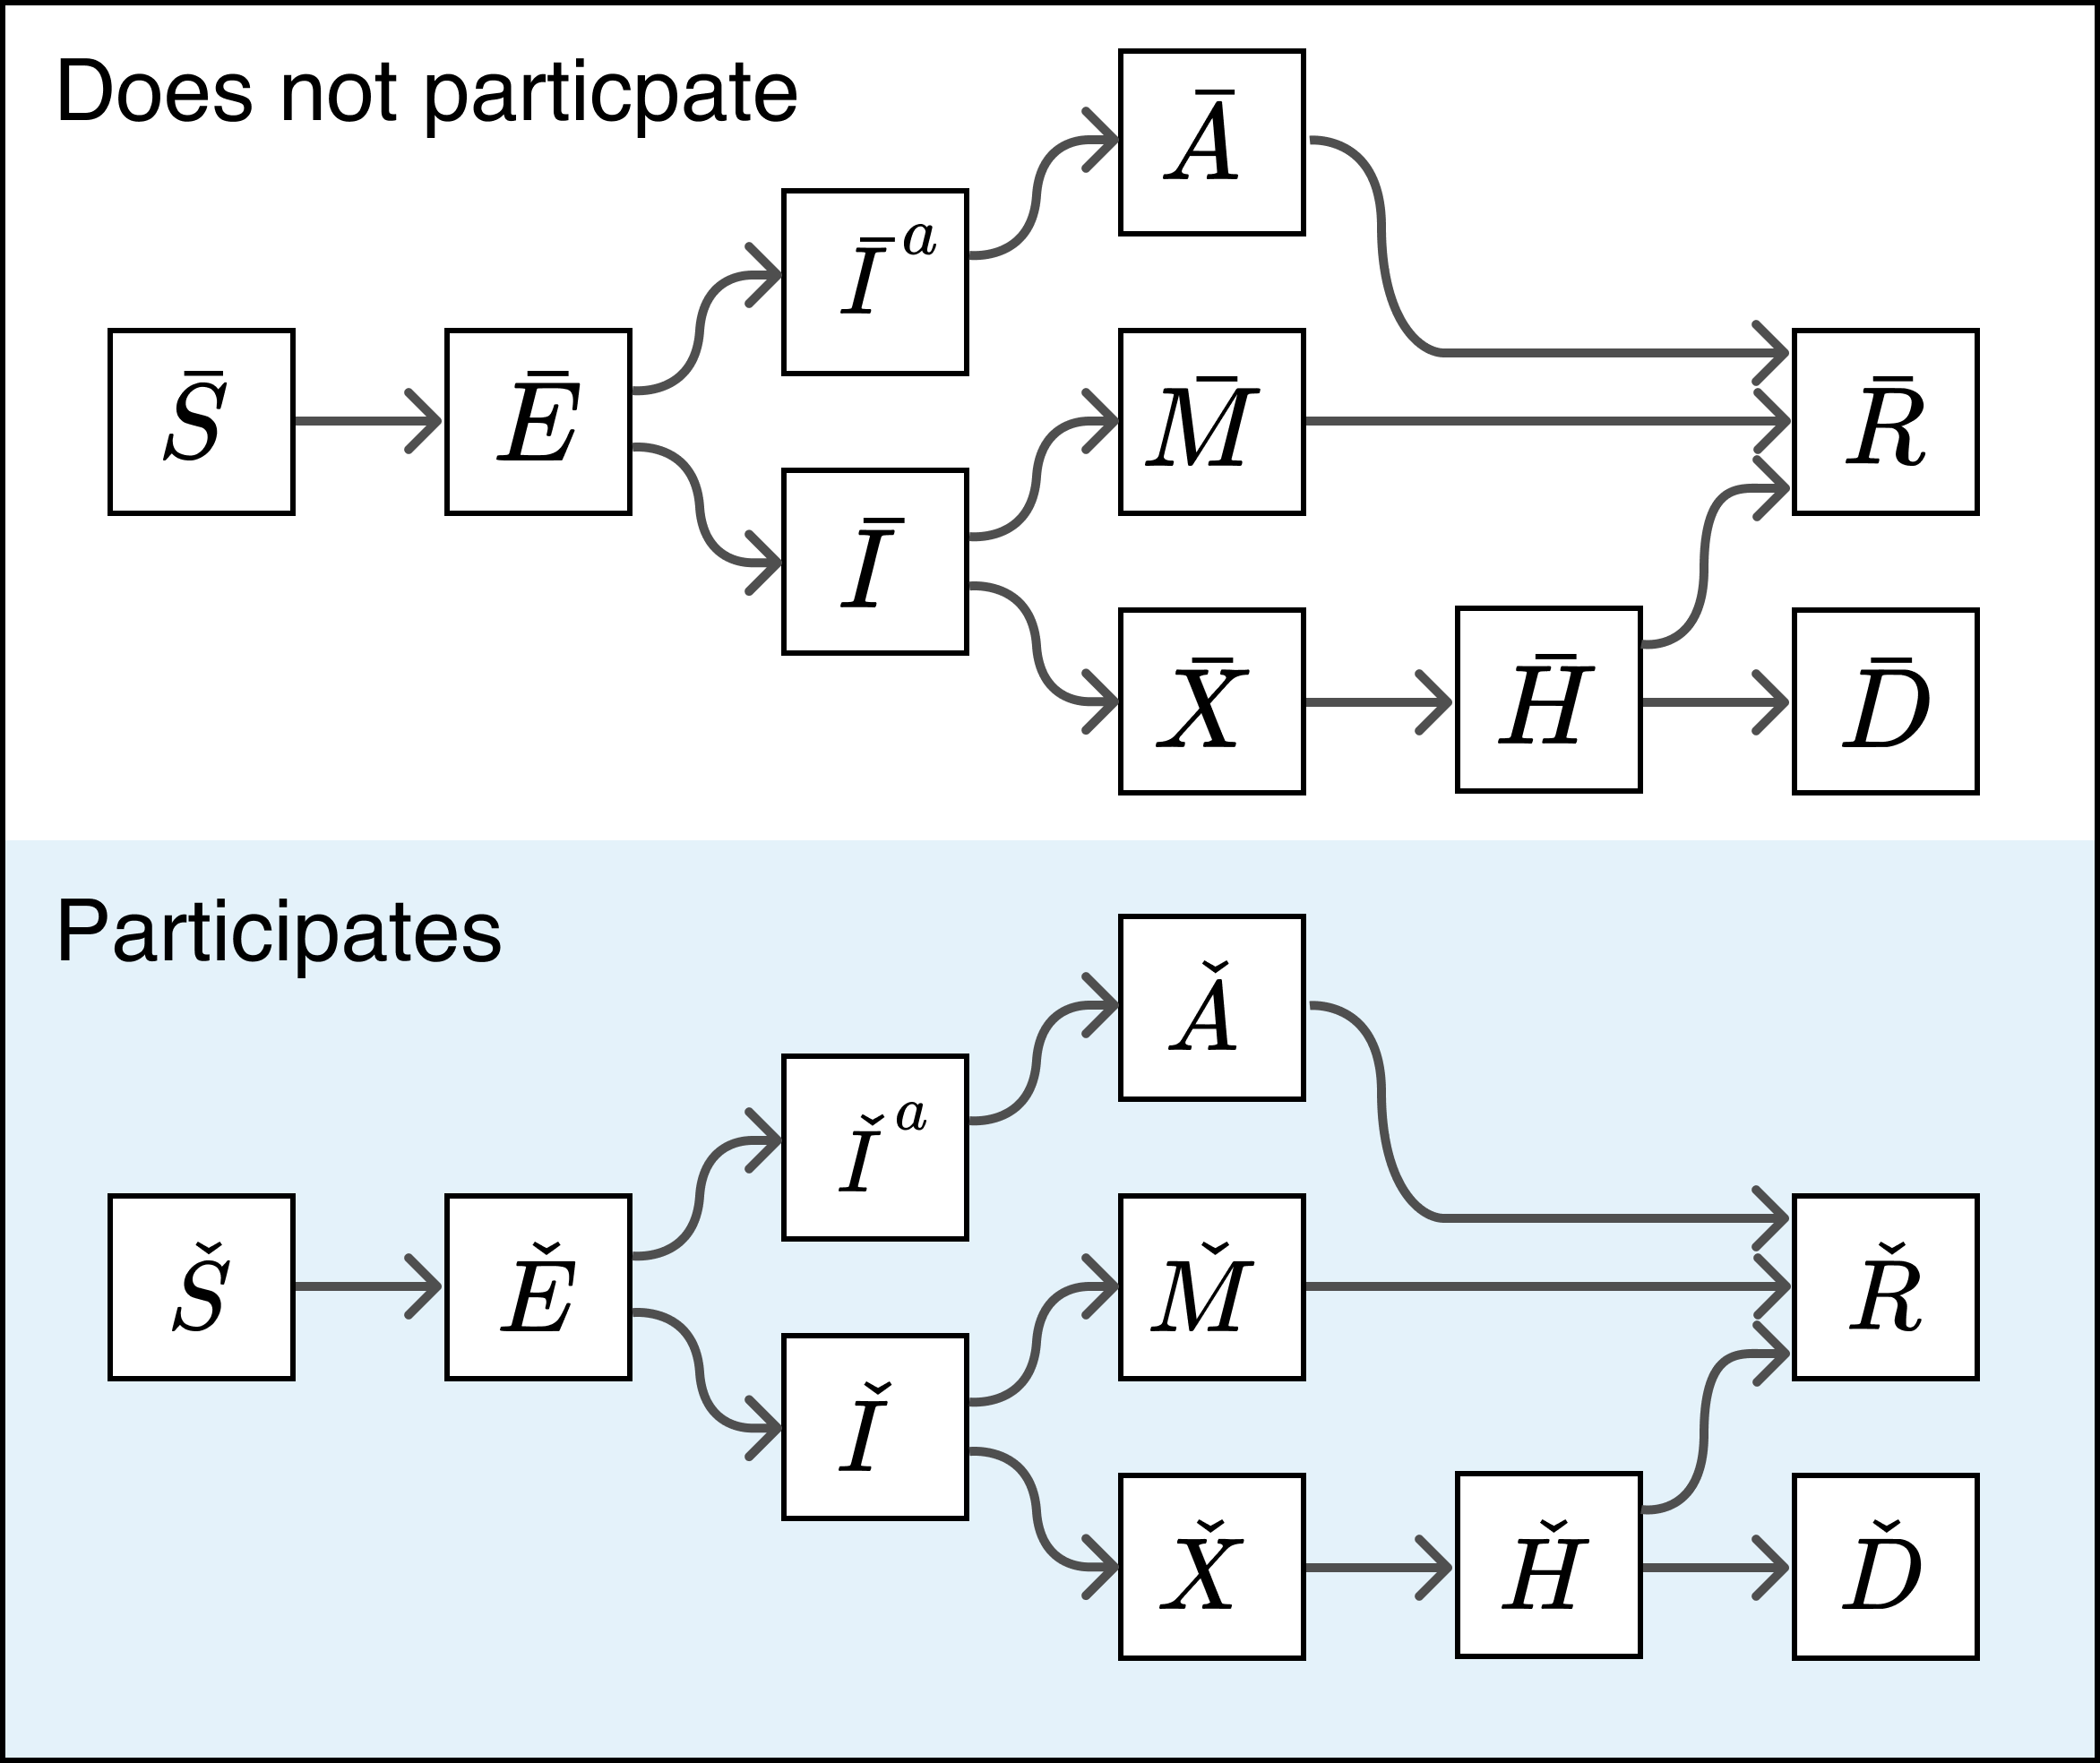
\includegraphics[width=3.5in]{SEIR with contact tracing}
\caption{\label{f:SEIR-contactSeparation}
 Those who chose not to participate in contact tracing and those that do particpate in contact tracing are treated separately. Population can never flow between the top and bottom graphs, although infectious individuals, regardless of whether they contact trace or not, can infect anyone who is suscpetible.}
\end{figure}

\begin{figure}
\centering
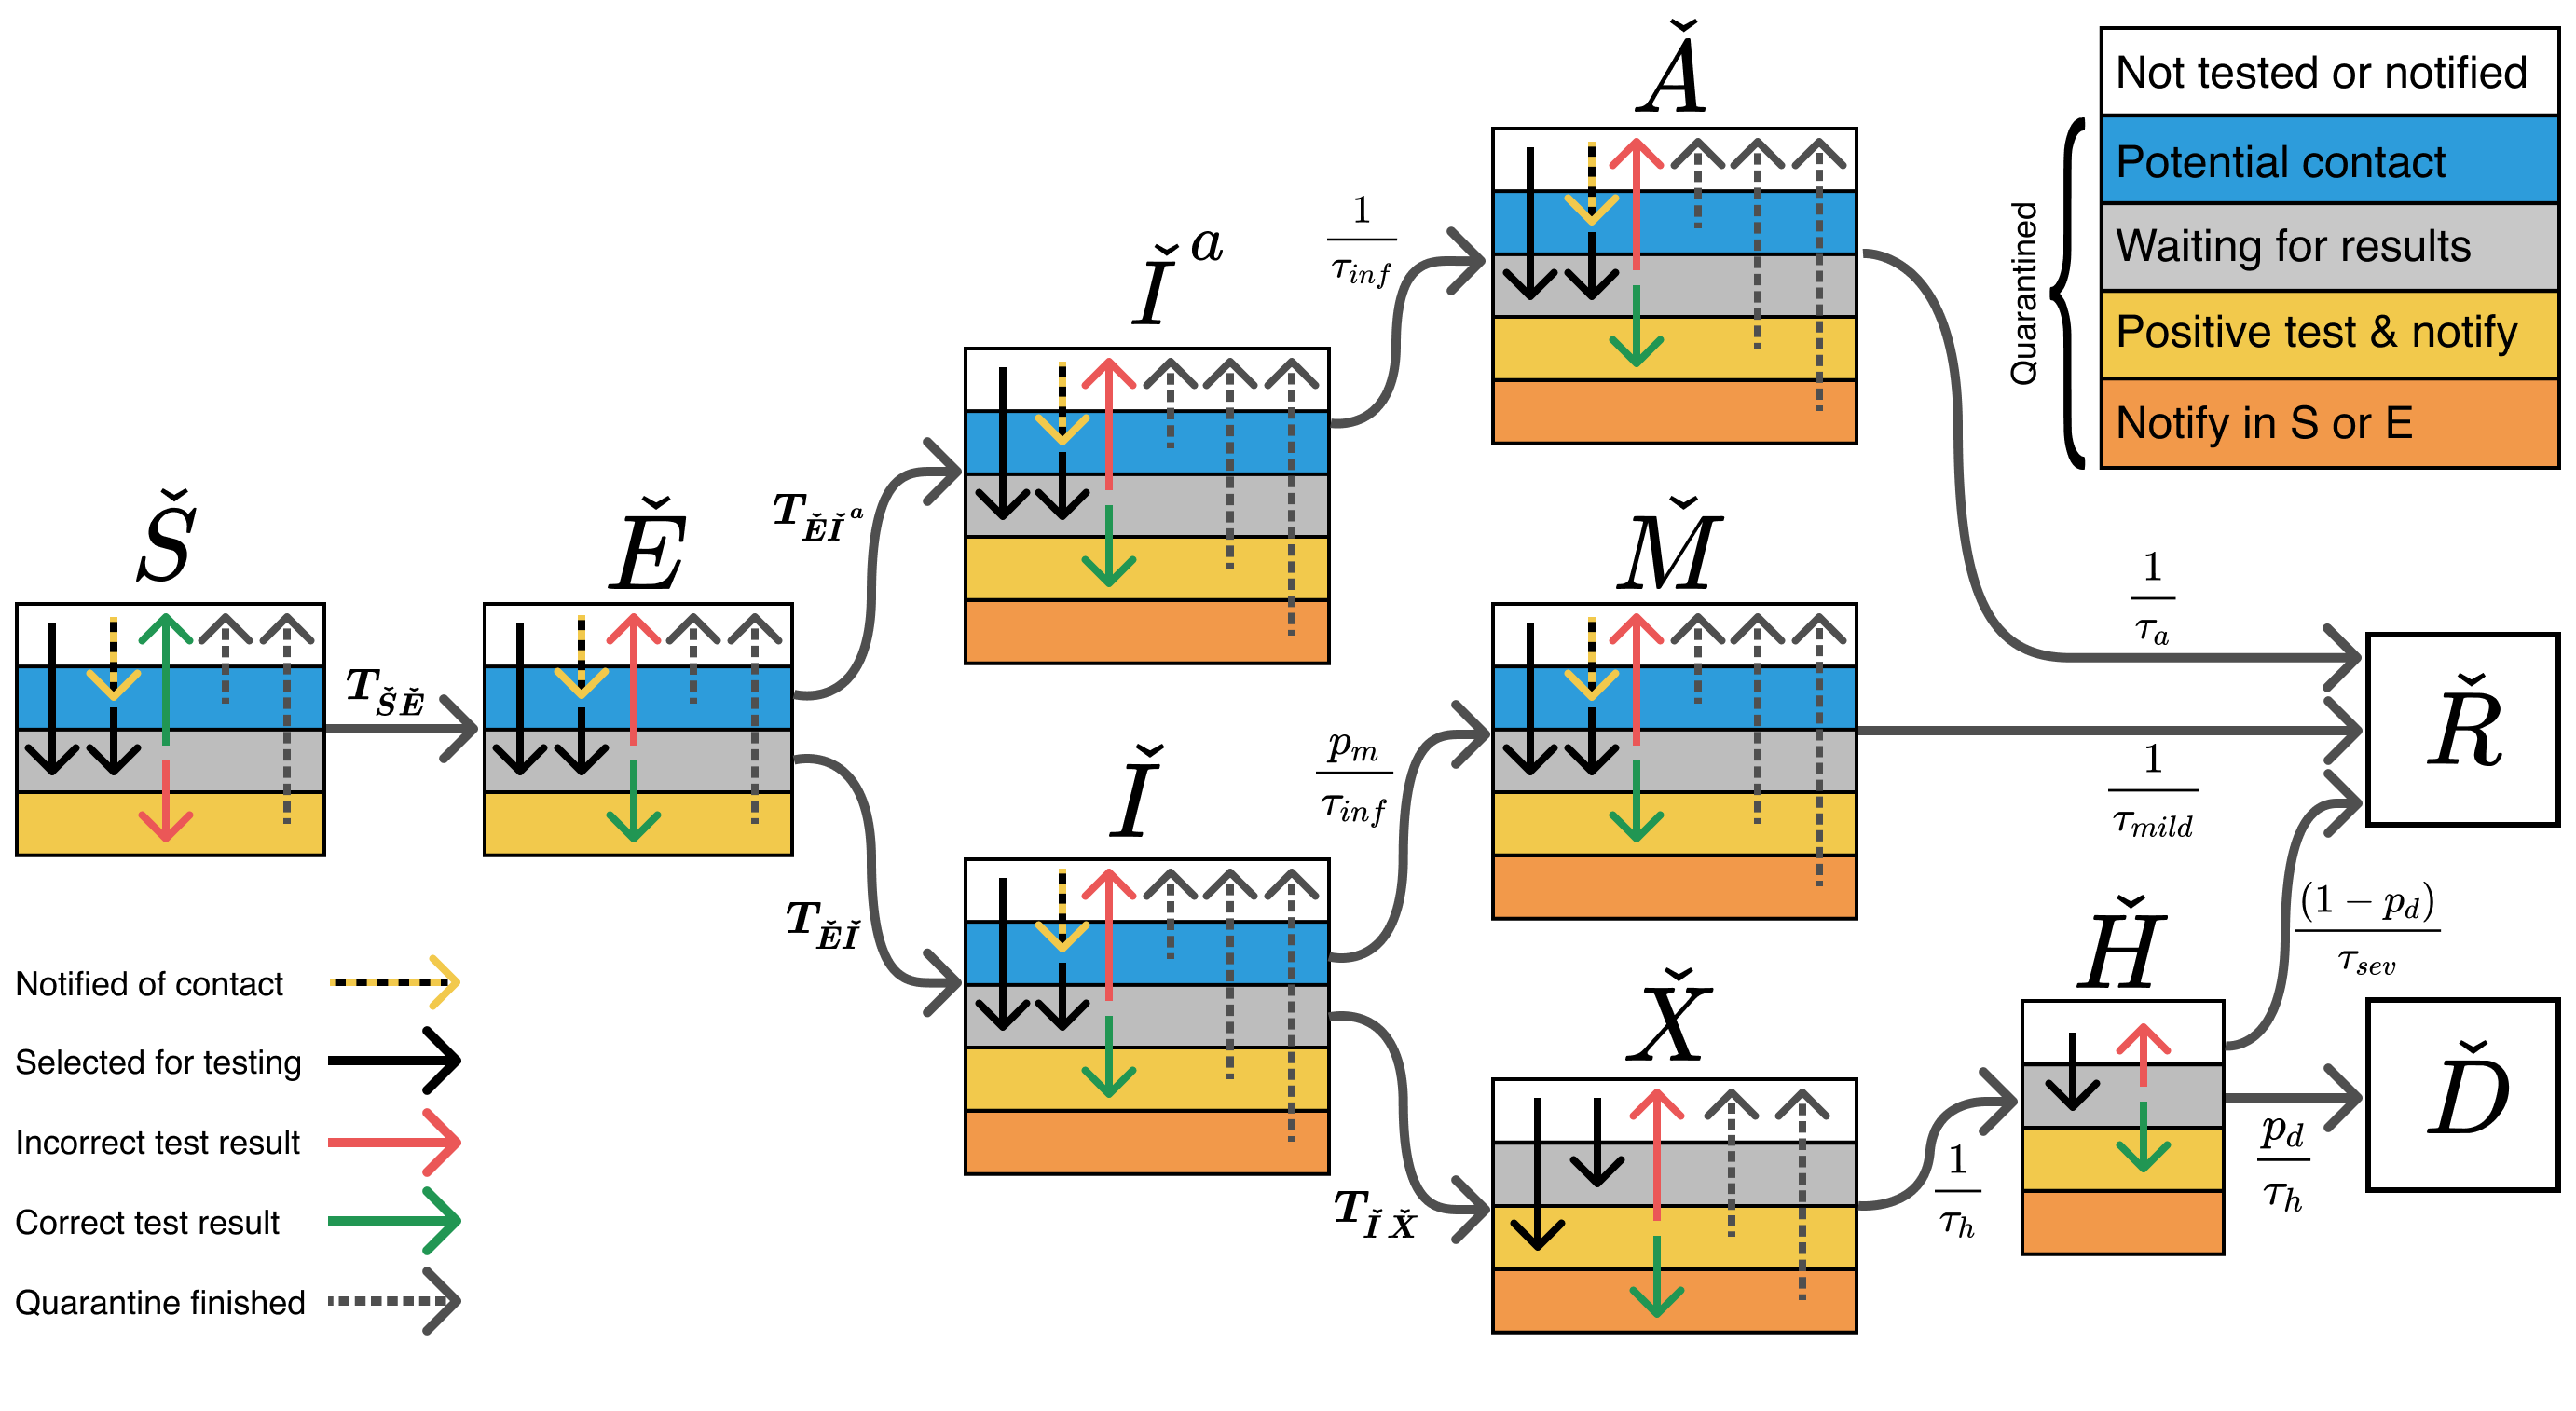
\includegraphics[width=6.5in]{SEIR_testing_and__contact_transitions}
\caption{\label{f:SEIR-contact}
 Layers for contact tracing, as well as the transition rates between populations.}
\end{figure}


% Here we introduce a new layer to the model that incorporates contact tracing. Contact tracing is a method of epidemic control that relies on tracing who those infected were in contact with, and then having them self-isolate. This reduces the spread of the disease as it is possible to identify and isolate those who are infectious as well as those who could potentially become infectious. Contact tracing relies on a large portion of the population participating as well as testing a substantial fraction of the population. Here we model the dynamics of contact tracing where $p_{c}$ is the fraction of the population who choose to participate, $p_t$ is the probability of an individual getting tested in a time interval $dt$, the tests take some time $\tau_{t}$ to process, and a person who tests positive and participates in contact tracing will on average notify the individuals they have been in contact with during the previous amount of time $\tau_{c}$. It is likely that those who participate in contact tracing and are notified that they may have been in contact with an infectious individual may be more likely to get tested. To account for this, those individuals may have a different probability of getting tested, $p^{c}_{t}$. A certain percentage of the tests performed will result in either a false positive ($f_{pos}$) or a false negative ($f_{neg}$). A simplified model of SEIR-C is shown in figure XXXX. Similar to SEIR, we will assume that the total population $N$ stays constant (births = deaths), and:
% \begin{eqnarray}
% \label{E:SEIRPop_c}
% N = S_{tot} + E_{tot} + I_{tot} + R_{tot}.
% \end{eqnarray}

% To simply matters, we assume that those who are tested immediately isolate themselves while waiting for the results. If a test comes back negative then they stop isolating, and if it is positive they continue isolating. Those that are infectious ($I_{iso}$), but isolating, will have a much smaller rate of passing on the infection $\beta_{iso} = \frac{R_{iso}}{\tau_{inf}}$, while those who are infectious but have not isolating ($I$) will remain infectious at a rate of $\beta_{0}$ used in the SEIR model. Anyone who has been exposed, but is now isolating either through a contact tracing notification or because they have been tested will eventually join $I_{iso}$ after an average time of $\tau_{inc}$. 


%%%%%%%%%%%%%%%%%%%%%%%%%%%%%%%%%%%%%%%%%%%%%%%%%%%%%%%%%
\section{Description of model}
%%%%%%%%%%%%%%%%%%%%%%%%%%%%%%%%%%%%%%%%%%%%%%%%%%%%%%%%%
Here we modify the SEIR model to include contact tracing and testing...

%%%%%%%%%%%%%%%%%%%%%%%%%%%%%%%%%%%%%%%%%%%%%%%%%%%%%%%%%
\subsection{Conventions and notation}
%%%%%%%%%%%%%%%%%%%%%%%%%%%%%%%%%%%%%%%%%%%%%%%%%%%%%%%%%
The populations are divided into those who particpate in contact tracing and those who do not. During each phase of the disease progression, there is never a transfer of popoulation from the group that is contact tracing and those who are not. We denote any population, $J$, that does not contact trace with a bar ($\bar{J}$) and those who do contact trace with a dot ($\check{J}$). 

In this model, anyone who is notified of a potential exposure through contact tracing is quarantined for some average time $\tau_{iso}$. During this time, their $R_{0}$ is reduced by a fraction $d_{r}$, making them far less likely to be exposed to the virus if they are susceptible, or much less likely to infect others if they are infectious. Testing can also take place. The average probability that someone in the general population is selected for testing is $p_{t}$. Later on we will allow for different testing rates for those who have been identified as being potentially exposed through contact tracing ($p^{c}_{t}$), those who show symptoms while infectious($p^{i}_{t}$), and those who develop severe symptoms ($p^{sev}_{t}$). We can also account for tests that return false positives ($f_{pos}$) and false negatives ($f_{neg}$), as well as the time it takes to get the test results ($\tau_{t}$) As in the basic SEIR model, the average time spent in the exposure phase is $\tau_{inc}$, and the time spend in the infectious phase is $\tau_{inf}$. Instead of a monolithic recovery phase, we consider several different subpopulations. There are those who are asymptomatic, those with mild infections, those with severe infections that lead to hospitalizations, and those who die after being hospitalized.

%%%%%%%%%%%%%%%%%%%%%%%%%%%%%%%%%%%%%%%%%%%%%%%%%%%%%%%%%
\section{Susceptible}
%%%%%%%%%%%%%%%%%%%%%%%%%%%%%%%%%%%%%%%%%%%%%%%%%%%%%%%%%
The rate of change equations for the susceptible populations that are not contact tracing ($\bar{S}$) are given as:
\begin{eqnarray}
\frac{d\bar{S}}{dt} &=& \boldsymbol{\bar{S}_{m}} \cdot  \bar{S}, 
\end{eqnarray}
where:
\begin{eqnarray}
\boldsymbol{\bar{S}_{m}} &=&
\begin{bmatrix}
-\gamma^{'} - p_{t}  &  \frac{(1-f_{pos})}{\tau_{t}}             & \frac{1}{\tau_{iso}} \\ 
 p_{t}              & -\frac{1}{\tau_{t}} - d_{r} \gamma^{'}    & 0  \\ 
 0                  & \frac{f_{pos}}{\tau_{t}}                  &  -d_{r} \gamma^{'}
\end{bmatrix} \\ 
%
\bar{S} &=& 
\begin{bmatrix}
\bar{S}_{g} \\ \bar{S}_{w}\\ \bar{S}_{t}
\end{bmatrix} \\
\end{eqnarray}
Here @TODO explain terms.

The rate of change of the susceptible populations that are particpating in contact tracing ($\check{S}$) are given as:
\begin{eqnarray}
\frac{d\check{S}}{dt} &=& \boldsymbol{\check{S}_{m}} \cdot \check{S},
\end{eqnarray}
where:
\begin{eqnarray}
\boldsymbol{\check{S}_{m}} &=&
\begin{bmatrix}
-\gamma^{'} -\gamma^{c}_{false} - p_{t}  & \frac{1}{\tau_{iso}}     & \frac{(1-f_{pos})}{\tau_{t}}             & \frac{1}{\tau_{iso}} \\ 
\gamma^{c}_{false}          &  -p^{c}_{t}  - \frac{1}{\tau_{iso}} -d_{r} \gamma^{'}          &  0    & 0  \\ 
p_{t}                          &  p^{c}_{t}                  &  -\frac{1}{\tau_{t}}  -d_{r} \gamma^{'}  & 0 \\
0 & 0 & \frac{f_{pos}}{\tau_{t}}  & -\frac{1}{\tau_{iso}}  -d_{r} \gamma^{'}
\end{bmatrix}, \\
% %
\check{S} &=& 
\begin{bmatrix}
\check{S}_{g} \\ \check{S}_{q} \\ \check{S}_{w}\\ \check{S}_{n}
\end{bmatrix}
\end{eqnarray}

%%%%%%%%%%%%%%%%%%%%%%%%%%%%%%%%%%%%%%%%%%%%%%%%%%%%%%%%%
\section{Exposure}
%%%%%%%%%%%%%%%%%%%%%%%%%%%%%%%%%%%%%%%%%%%%%%%%%%%%%%%%%
The rate of change equations for the exposed populations that are not contact tracing ($\bar{S}$) are given as:
\begin{eqnarray}
\frac{d\bar{E}}{dt} &=& \boldsymbol{\bar{E}_{m}} \cdot \bar{E} + \boldsymbol{T_{\bar{S}\bar{E}}}  \bar{S}, 
\end{eqnarray}
where:
\begin{eqnarray}
\boldsymbol{\bar{E}_{m}} &=&
\begin{bmatrix}
 - p_{t} -\frac{1}{\tau_{inc}}  &  \frac{(1-f_{neg})}{\tau_{t}}             & \frac{1}{\tau_{iso}} \\ 
 p_{t}              & -\frac{1}{\tau_{t}} -\frac{1}{\tau_{inc}}  & 0  \\ 
 0                  & \frac{f_{neg}}{\tau_{t}}                  & -\frac{1}{\tau_{iso}} -\frac{1}{\tau_{inc}}
\end{bmatrix} \\ 
%
\bar{E} &=& 
\begin{bmatrix}
\bar{E}_{g} \\ \bar{E}_{w}\\ \bar{E}_{t}
\end{bmatrix} \\
%
\boldsymbol{T_{\bar{S}\bar{E}}} &=& 
    \begin{bmatrix}
\gamma^{'}  & 0                 & 0 \\ 
 0          & d_{r} \gamma^{'}  & 0 \\ 
 0          & 0                 & d_{r} \gamma^{'} 
\end{bmatrix}.
%
\end{eqnarray}

For the exposedß population particpating in contact tracing we have:
\begin{eqnarray}
\frac{d\check{E}}{dt} &=& \boldsymbol{\check{E}_{m}} \cdot \check{E} + \boldsymbol{T_{\check{S}\check{E}}}  \check{S}, 
\end{eqnarray}
where:
\begin{eqnarray}
\boldsymbol{\check{E}_{m}} &=&
\begin{bmatrix}
 -\gamma^{c}_{false} -\gamma^{c}_{true} - p_{t} -\frac{1}{\tau_{inc}} & \frac{1}{\tau_{iso}}  & \frac{f_{neg}}{\tau_{t}} & \frac{1}{\tau_{iso}} \\
\gamma^{c}_{false} + \gamma^{c}_{true}    &  -p^{c}_{t}  - \frac{1}{\tau_{iso}} - \frac{1}{\tau_{inc}}      &  0    & 0  \\
p_{t}     &  p^{c}_{t}                  &  -\frac{1}{\tau_{t}}  - \frac{1}{\tau_{inc}}  & 0 \\
0 & 0 & \frac{(1-f_{neg})}{\tau_{t}}  & -\frac{1}{\tau_{iso}}  -  \frac{1}{\tau_{inc}} 
\end{bmatrix}, \\ 
%
\check{E} &=& 
\begin{bmatrix}
\check{E}_{g} \\ \check{E}_{q} \\ \check{E}_{w}\\ \check{E}_{n}
\end{bmatrix}, \\ 
%
\boldsymbol{T_{\check{S}\check{E}}} &=&
\begin{bmatrix}
\gamma^{'}  & 0                 & 0                 & 0 \\ 
 0          & d_{r} \gamma^{'}  & 0                 & 0 \\ 
 0          & 0                 & d_{r} \gamma^{'}  & 0  \\
 0          & 0                 & 0                 & d_{r} \gamma^{'}
\end{bmatrix}.
\end{eqnarray}


%%%%%%%%%%%%%%%%%%%%%%%%%%%%%%%%%%%%%%%%%%%%%%%%%%%%%%%%%
\section{Infectious}
%%%%%%%%%%%%%%%%%%%%%%%%%%%%%%%%%%%%%%%%%%%%%%%%%%%%%%%%%
In the infectious population, we must consider that a certain percentage of those infected ($p_{a}$) will be asymptomatic. Those who display no symptoms will not be as likely to be tested, and will be more difficult to quarantine. The asymptomatic individuals will be split between those who contact trace and those who do not. We denote those who are asymptomatic with a superscript $a$. 

%%%%%%%%%%%%%%%%%%%%%%%%%%%%%%%%%%%%%%%%%%%%%%%%%%%%%%%%%
\subsection{Individuals who are infectious and display symptoms}
%%%%%%%%%%%%%%%%%%%%%%%%%%%%%%%%%%%%%%%%%%%%%%%%%%%%%%%%%
First we consider those who display symptoms, but don't contact trace:
\begin{eqnarray}
\frac{d\bar{I}}{dt} &=& \boldsymbol{\bar{I}_{m}} \cdot  \bar{I} + \frac{(1-p_{a})}{\tau_{inc}} \mathbb{1} \cdot \bar{E}, 
\end{eqnarray}
where:
%
\begin{eqnarray}
\boldsymbol{\bar{I}_{m}} &=&
\begin{bmatrix}
- p^{i}_{t} -\frac{1}{\tau_{inf}}  &  \frac{f_{neg}}{\tau_{t}}            & \frac{1}{\tau_{iso}} \\ 
 p^{i}_{t}              & -\frac{1}{\tau_{t}} -\frac{1}{\tau_{inf}}       & 0  \\ 
 0                  & \frac{(1- f_{neg})}{\tau_{t}}                        & -\frac{1}{\tau_{iso}} -\frac{1}{\tau_{inf}}
\end{bmatrix}, \\ 
%
\bar{I} &=& 
\begin{bmatrix}
\bar{I}_{g} \\ \bar{I}_{w}\\ \bar{I}_{t}
\end{bmatrix}, \\ 
%
% \boldsymbol{T_{\bar{E}\bar{I}}} &=&
% \begin{bmatrix}
% \frac{(1-p_{a})}{\tau_{inc}}  & 0                 & 0 \\ 
%  0          &  \frac{(1-p_{a})}{\tau_{inc}}  & 0 \\ 
%  0          & 0                 &  \frac{(1-p_{a})}{\tau_{inc}} 
% \end{bmatrix}.
%
\end{eqnarray}
and the idenity matrix is represented as $\mathbb{1}$.

Those who particpate in contact tracing, are infectious, and display symptoms:
\begin{eqnarray}
\frac{d\check{I}}{dt} &=& \boldsymbol{\check{I}_{m}}  \check{I} + \boldsymbol{T_{\check{E}\check{I}}} \cdot  \check{E}, 
\end{eqnarray}
where:
%
\begin{eqnarray}
\boldsymbol{\check{I}_{m}} &=&
\begin{bmatrix}
 -\gamma^{c}_{false} -\gamma^{c}_{true} - p^{i}_{t} -\frac{1}{\tau_{inf}} & \frac{1}{\tau_{iso}}  & \frac{f_{neg}}{\tau_{t}} & \frac{1}{\tau_{iso}} & \frac{1}{\tau_{iso}} \\
 %
\gamma^{c}_{false} + \gamma^{c}_{true}    &  -p^{n}_{t}  - \frac{1}{\tau_{iso}} - \frac{1}{\tau_{inf}}      &  0    & 0  & 0\\
p^{i}_{t}     &  p^{n}_{t}                  &  -\frac{1}{\tau_{t}}  - \frac{1}{\tau_{inf}}  & 0 & 0\\
0 & 0 & \frac{(1-f_{neg})}{\tau_{t}}  & -\frac{1}{\tau_{iso}}  -  \frac{1}{\tau_{inf}} & 0 \\ 
0 & 0 & 0 & 0 & -\frac{1}{\tau_{iso}}  -  \frac{1}{\tau_{inf}}
\end{bmatrix}, \\ 
%
\check{I} &=& 
\begin{bmatrix}
\check{I}_{g} \\ \check{I}_{q} \\ \check{I}_{w}\\ \check{I}_{n} \\ \check{I}_{n'}
\end{bmatrix}, \\
%
\boldsymbol{T_{\check{E}\check{I}}} &=& \frac{(1-p_{a})}{\tau_{inc}} 
\begin{bmatrix}
1  & 0 & 0 & 0 & 0\\ 
0  & 1 & 0 & 0 & 0 \\ 
0  & 0 & 1 & 0 & 0 \\ 
0  & 0 & 0 & 0 & 0 \\ 
0  & 0 & 0 & 1 & 0 
\end{bmatrix}.
\end{eqnarray}

%%%%%%%%%%%%%%%%%%%%%%%%%%%%%%%%%%%%%%%%%%%%%%%%%%%%%%%%%
\subsection{Asymptomatic}
%%%%%%%%%%%%%%%%%%%%%%%%%%%%%%%%%%%%%%%%%%%%%%%%%%%%%%%%%
For those who are asymptomatic, we first look at the group that does not particpate in contact tracing:
\begin{eqnarray}
\frac{d\bar{I}^{a}}{dt} &=& \boldsymbol{\bar{I}^{a}_{m}} \cdot \bar{I}^{a} + \frac{p_{a}}{\tau_{inc}} \mathbb{1} \cdot  \bar{E}, \\ 
\boldsymbol{\bar{I}^{a}_{m}} &=& \boldsymbol{\bar{I}_{m}}, \\ 
%
\bar{I}^{a} &=& 
\begin{bmatrix}
\bar{I}^{a}_{g} \\ \bar{I}^{a}_{w}\\ \bar{I}^{a}_{t}
\end{bmatrix},
\end{eqnarray}
% where:
% %
% \begin{eqnarray}
% \boldsymbol{\bar{I}^{a}_{m}} &=& \boldsymbol{\bar{I}_{m}}, \\ 
% %
% \bar{I}^{a} &=& 
% \begin{bmatrix}
% \bar{I}^{a}_{g} \\ \bar{I}^{a}_{w}\\ \bar{I}^{a}_{t}
% \end{bmatrix}, \\ 
% %
% % \boldsymbol{T_{\bar{E}\bar{I}^{a}}} &=&
% % \begin{bmatrix}
% % \frac{p_{a}}{\tau_{inc}}  & 0                 & 0 \\ 
% %  0          &  \frac{p_{a}}{\tau_{inc}}  & 0 \\ 
% %  0          & 0                 &  \frac{p_{a}}{\tau_{inc}} 
% % \end{bmatrix}.
% \end{eqnarray}



Finally, we have those who are asymptomatic but are particpating in contact tracing:
\begin{eqnarray}
\frac{d\check{I}^{a}}{dt} &=& \boldsymbol{\check{I}^{a}_{m}} \cdot \check{I}^{a} + \boldsymbol{T_{\check{E}\check{I}^{a}}} \cdot  \check{E}, \\
\boldsymbol{\check{I}^{a}_{m}} &=& \boldsymbol{\check{I}_{m}}, \\ 
%
\boldsymbol{T_{\check{E}\check{I}^{a}}} &=& \boldsymbol{T_{\bar{E}\bar{I}^{a}}} \\
%
\check{I} &=& 
\begin{bmatrix}
\check{I}^{a}_{g} \\[.15cm] \check{I}^{a}_{q} \\[.15cm] \check{I}^{a}_{w}\\[.15cm] \check{I}^{a}_{n} \\[.15cm] \check{I}^{a}_{n'}
\end{bmatrix}
\end{eqnarray}
% %
% \begin{eqnarray}
% \boldsymbol{\check{I}^{a}_{m}} &=& \boldsymbol{\check{I}_{m}}, \\ 
% %
% % \boldsymbol{T_{\check{E}\check{I}^{a}}} &=&
% % \begin{bmatrix}
% % \frac{p_{a}}{\tau_{inc}}  & 0                 & 0 & 0 & 0\\ 
% %  0          &  \frac{p_{a}}{\tau_{inc}}  & 0 & 0 & 0 \\ 
% %  0          & 0                 &  \frac{p_{a}}{\tau_{inc}} & 0 & 0 \\ 
% % 0           & 0                 &  0 & 0 & 0 \\ 
% % 0           & 0                 &  0 & \frac{p_{a}}{\tau_{inc}} & 0 \\
% % \end{bmatrix}
% \end{eqnarray}


%%%%%%%%%%%%%%%%%%%%%%%%%%%%%%%%%%%%%
\section{Outcomes}
%%%%%%%%%%%%%%%%%%%%%%%%%%%%%%%%%%%%%
This is part of the $R$ section in a traditional $SEIR$ model. We divide this into several transition times as it make take a patient some time to recover after they are infectious (and therefore still test positive). We divide these up into those who are asymptomatic, mild, and severe. Those who are severe have a chance $p_h$ of needing hospitalization or making a recovery $R$. Those who are hospitalized can recover $R$ or die $D$. We denote the intermetiate states where someone is in the recovery process $O$ for outcomes.

%%%%%%%%%%%%%%%%%%%%%%%%%%%%%%%%%%%%%
\subsection{Asymptomatic}
%%%%%%%%%%%%%%%%%%%%%%%%%%%%%%%%%%%%%
Those who are asymptomatic, but not particpating in contact tracing, have a population that changes:
\begin{eqnarray}
\frac{d\bar{A}}{dt} &=& \boldsymbol{\bar{A}_{m}} \cdot  \bar{A} + \frac{1}{\tau_{inf}} \mathbb{1} \cdot  \bar{I}^{a}, 
\end{eqnarray}
where:
%
\begin{eqnarray}
\boldsymbol{\bar{A}_{m}} &=&
\begin{bmatrix}
- p_{t} -\frac{1}{\tau_{a}}  &  \frac{f_{neg}}{\tau_{t}}            & \frac{1}{\tau_{iso}} \\ 
 p_{t}              & -\frac{1}{\tau_{t}} -\frac{1}{\tau_{a}}       & 0  \\ 
 0                  & \frac{(1- f_{neg})}{\tau_{t}}                        & -\frac{1}{\tau_{iso}} -\frac{1}{\tau_{a}}
\end{bmatrix}, \\ 
%
\bar{A} &=& 
\begin{bmatrix}
\bar{A}_{g} \\ \bar{A}_{w}\\ \bar{A}_{t}
\end{bmatrix}. \\ 
%
% \boldsymbol{T_{\bar{I}\bar{A}}} &=&
% \begin{bmatrix}
% \frac{1}{\tau_{inf}}  & 0                 & 0 \\ 
%  0          &  \frac{1}{\tau_{inf}}  & 0 \\ 
%  0          & 0                 &  \frac{1}{\tau_{inf}} 
% \end{bmatrix}.
% %
\end{eqnarray}

Those who are participating in contact tracing, but are asymptomatic have the following population change as a function of time:
\begin{eqnarray}
\frac{d\check{A}}{dt} &=& \boldsymbol{\check{A}_{m}} \cdot  \check{A} + \frac{1}{\tau_{inf}} \mathbb{1} \cdot  \check{I}^{a}, 
\end{eqnarray}
where:
%
\begin{eqnarray}
\boldsymbol{\check{A}_{m}}&=&
\begin{bmatrix}
 -\gamma^{c}_{false} -\gamma^{c}_{true} - p_{t} -\frac{1}{\tau_{a}} & \frac{1}{\tau_{iso}}  & \frac{f_{neg}}{\tau_{t}} & \frac{1}{\tau_{iso}} & \frac{1}{\tau_{iso}} \\
 %
\gamma^{c}_{false} + \gamma^{c}_{true}    &  -p^{c}_{t}  - \frac{1}{\tau_{iso}} - \frac{1}{\tau_{a}}      &  0    & 0  & 0\\
p_{t}     &  p^{c}_{t}                  &  -\frac{1}{\tau_{t}}  - \frac{1}{\tau_{a}}  & 0 & 0\\
0 & 0 & \frac{(1-f_{neg})}{\tau_{t}}  & -\frac{1}{\tau_{iso}}  -  \frac{1}{\tau_{a}} & 0 \\ 
0 & 0 & 0 & 0 & -\frac{1}{\tau_{iso}}  -  \frac{1}{\tau_{a}}
\end{bmatrix}, \\ 
%
\check{A} &=& 
\begin{bmatrix}
\check{A}_{g} \\ \check{A}_{q} \\ \check{A}_{w}\\ \check{A_{n}} \\ \check{A_{n'}}
\end{bmatrix}. \\ 
%
% 
% \boldsymbol{T_{\check{I}\check{A}}} &=&
% \begin{bmatrix}
% \frac{1}{\tau_{inf}}  & 0                 & 0 & 0 & 0\\ 
%  0          &  \frac{1}{\tau_{inf}}  & 0 & 0 & 0 \\ 
%  0          & 0                 &  \frac{1}{\tau_{inf}} & 0 & 0 \\ 
% 0           & 0                 &  0 & \frac{1}{\tau_{inf}} & 0 \\ 
% 0           & 0                 &  0 & 0 & \frac{1}{\tau_{inf}} \\
% \end{bmatrix}
\end{eqnarray}
We must track each of these subpopulations. Even though no one in $A$ is still infectious, they can still test positive and thereby notify others that they need to quarantine themselves (including those who they may have infected). 

% Now we look at the transition matrix from those who are infectious but asymptomatic to those awaiting their outcome who are asymptomatic. For those not participating in contact tracing, the matrix is:
% \begin{eqnarray}
% T_{\bar{I^{a}} \rightarrow \bar{A}} &=&
% \begin{bmatrix}
% \frac{1}{\tau_{inf}}  & 0                 & 0 \\ 
%  0          &  \frac{1}{\tau_{inf}}  & 0 \\ 
%  0          & 0                 &  \frac{1}{\tau_{inf}} 
% \end{bmatrix}.
% \end{eqnarray}
% For those who particpate in contact tracing and are asymptomatic move from infectious to outcomes with the following transition matrix: 
% Transition Econ -> Icon participating in contact (asymptomatic)
% \begin{eqnarray}
% T_{\check{I}^{a} \rightarrow \check{A}} &=&
% \begin{bmatrix}
% \frac{1}{\tau_{inf}}  & 0                 & 0 & 0 & 0\\ 
%  0          &  \frac{1}{\tau_{inf}}  & 0 & 0 & 0 \\ 
%  0          & 0                 &  \frac{1}{\tau_{inf}} & 0 & 0 \\ 
% 0           & 0                 &  0 & \frac{1}{\tau_{inf}} & 0 \\ 
% 0           & 0                 &  0 & 0 & \frac{1}{\tau_{inf}} \\
% \end{bmatrix}
% \end{eqnarray}

%%%%%%%%%%%%%%%%%%%%%%%%%%%%%%%%%%%%%
\subsubsection{Mild}
%%%%%%%%%%%%%%%%%%%%%%%%%%%%%%%%%%%%%
We now deal with the infectious population who develop a mild case (show symptoms), but do not need hospitalization and do not die. These individual recover in a time $\tau_{mild}$, and make up $p_{mild}$ fraction of total infectious cases. Asymptomatic individuals cannot be included in this group. Since we are looking at a subpoulation who aren't asymptomatic, we must account for this. The fraction of nonasymptomatic individuals who develop mild cases is given as:
\begin{eqnarray}
p_{m} &=& \frac{p_{mild}}{(1 - p_{a})}. 
\end{eqnarray}

For those who develop mild cases and do not particpate in contact tracing we have:
\begin{eqnarray}
\frac{d\bar{M}}{dt} &=& \boldsymbol{\bar{M}_{m}} \cdot \bar{M} + \frac{p_{m}}{\tau_{inf}} \mathbb{1} \cdot  \bar{I}, 
\end{eqnarray}
where:
%
\begin{eqnarray}
\boldsymbol{\bar{M}_{m}} &=&
\begin{bmatrix}
- p_{t} -\frac{1}{\tau_{mild}}  &  \frac{f_{neg}}{\tau_{t}}            & \frac{1}{\tau_{iso}} \\ 
 p_{t}              & -\frac{1}{\tau_{t}} -\frac{1}{\tau_{mild}}       & 0  \\ 
 0                  & \frac{(1- f_{neg})}{\tau_{t}}                        & -\frac{1}{\tau_{iso}} -\frac{1}{\tau_{mild}}
\end{bmatrix}, \\ 
%
\bar{M} &=& 
\begin{bmatrix}
\bar{M}_{g} \\ \bar{M}_{w}\\ \bar{M}_{t}
\end{bmatrix}. \\ 
%
%T_{\bar{I} \rightarrow \bar{M}} 
% \boldsymbol{T_{\bar{I}\bar{M}}}&=&
% \begin{bmatrix}
% \frac{p_{m}}{\tau_{inf}}  & 0                 & 0 \\ 
%  0          &  \frac{p_{m}}{\tau_{inf}}  & 0 \\ 
%  0          & 0                 &  \frac{p_{m}}{\tau_{inf}} 
% \end{bmatrix}.
%
\end{eqnarray} 

Finally, for those who develop mild cases and contact trace:
\begin{eqnarray}
\frac{d\check{M}}{dt} &=& \boldsymbol{\check{M}_{m}} \cdot \check{M} + \frac{p_{m}}{\tau_{inf}} \mathbb{1} \cdot  \check{I}, 
\end{eqnarray}
where:
%
\begin{eqnarray}
\boldsymbol{\check{M}_{m}} &=&
\begin{bmatrix}
 -\gamma^{c}_{false} -\gamma^{c}_{true} - p_{t} -\frac{1}{\tau_{mild}} & \frac{1}{\tau_{iso}}  & \frac{f_{neg}}{\tau_{t}} & \frac{1}{\tau_{iso}} & \frac{1}{\tau_{iso}} \\
 %
\gamma^{c}_{false} + \gamma^{c}_{true}    &  -p^{c}_{t}  - \frac{1}{\tau_{iso}} - \frac{1}{\tau_{mild}}      &  0    & 0  & 0\\
p_{t}     &  p^{c}_{t}                  &  -\frac{1}{\tau_{t}}  - \frac{1}{\tau_{mild}}  & 0 & 0\\
0 & 0 & \frac{(1-f_{neg})}{\tau_{t}}  & -\frac{1}{\tau_{iso}}  -  \frac{1}{\tau_{mild}} & 0 \\ 
0 & 0 & 0 & 0 & -\frac{1}{\tau_{iso}}  -  \frac{1}{\tau_{mild}}
\end{bmatrix}, \\ 
%
\check{M} &=& 
\begin{bmatrix}
\check{M}_{g} \\ \check{M}_{q} \\ \check{M}_{w}\\ \check{M_{n}} \\ \check{M_{n'}}
\end{bmatrix}. \\ 
%
% \boldsymbol{T_{\check{I}\check{M}}} &=&
% \begin{bmatrix}
% \frac{p_{m}}{\tau_{inf}}  & 0                 & 0 & 0 & 0\\ 
%  0          &  \frac{p_{m}}{\tau_{inf}}  & 0 & 0 & 0 \\ 
%  0          & 0                 &  \frac{p_{m}}{\tau_{inf}} & 0 & 0 \\ 
% 0           & 0                 &  0 & \frac{p_{m}}{\tau_{inf}} & 0 \\ 
% 0           & 0                 &  0 & 0 & \frac{p_{m}}{\tau_{inf}} \\
% \end{bmatrix}.
%
\end{eqnarray}



%%%%%%%%%%%%%%%%%%%%%%%%%%%%%%%%%%%%%%%%
\subsection{Severe}
%%%%%%%%%%%%%%%%%%%%%%%%%%%%%%%%%%%%%%%%
The final group we must consider are those who are severe cases. These represent the following fraction of the symptomatic cases that are severe:
\begin{eqnarray}
p_{sev} &=& 1 - p_{m},
\end{eqnarray}
and lead to hospitalization some time $\tau_{h}$ after they cease to be infectious. We also assume that anyone in the severe category will be tested at a rate $p^{sev}_{t}$ regardless of whether they have been notified of a potential contact Those hospitalized will either recover or die. Those who do not particpate in contact tracing can be descibed by the following dynamics:
\begin{eqnarray}
\frac{d\bar{X}}{dt} &=& \boldsymbol{\bar{X}_{m}} \cdot \bar{X} + \frac{p_{sev}}{\tau_{inf}} \mathbb{1} \cdot  \bar{I}, 
\end{eqnarray}
where:
%
\begin{eqnarray}
\boldsymbol{\bar{X}_{m}} &=&
\begin{bmatrix}
- p^{sev}_{t} -\frac{1}{\tau_{h}}  &  \frac{f_{neg}}{\tau_{t}}            & \frac{1}{\tau_{iso}} \\ 
 p^{sev}_{t}              & -\frac{1}{\tau_{t}} -\frac{1}{\tau_{h}}       & 0  \\ 
 0                  & \frac{(1- f_{neg})}{\tau_{t}}                        & -\frac{1}{\tau_{iso}} -\frac{1}{\tau_{h}}
\end{bmatrix}, \\ 
%
\bar{X} &=& 
\begin{bmatrix}
\bar{X}_{g} \\ \bar{X}_{w}\\ \bar{X}_{t}
\end{bmatrix}. \\ 
%
% \boldsymbol{T_{\bar{I}\bar{X}}} &=&
% \begin{bmatrix}
% \frac{p_{sev}}{\tau_{inf}}  & 0                 & 0 \\ 
%  0          &  \frac{p_{}}{\tau_{inf}}  & 0 \\ 
%  0          & 0                 &  \frac{p_{}}{\tau_{inf}} 
% \end{bmatrix}.
% %
\end{eqnarray}

For those who do particpate in contact tracing but develop severe symptoms we have:
\begin{eqnarray}
\frac{d\check{X}}{dt} &=& \boldsymbol{\check{X}_{m}} \cdot  \check{X} + \frac{p_{sev}}{\tau_{inf}} \mathbb{1} \cdot  \check{I}, 
\end{eqnarray}
where:
%
\begin{eqnarray}
\boldsymbol{\check{X}_{m}} &=&
\begin{bmatrix}
 %
- p^{sev}_{t}   - \frac{1}{\tau_{h}}      &  \frac{f_{neg}}{\tau_{t}}    & 0  & 0\\
p^{sev}_{t}                  &  -\frac{1}{\tau_{t}}  - \frac{1}{\tau_{h}}  & 0 & 0\\
0 & \frac{(1-f_{neg})}{\tau_{t}}  &  -  \frac{1}{\tau_{h}} & 0 \\ 
0 & 0 & 0 &  -  \frac{1}{\tau_{h}}
\end{bmatrix}, \\ 
%
\check{X} &=& 
\begin{bmatrix}
\check{X}_{g} \\  \check{X}_{w}\\ \check{X_{n}} \\ \check{X_{n'}}
\end{bmatrix}, \\ 
%
\boldsymbol{T_{\check{I}\check{X}}} &=& \frac{p_{sev}}{\tau_{inf}}
\begin{bmatrix}
1  & 1 & 0 & 0 & 0 \\ 
0  & 0 & 0 & 0 & 0 \\ 
0  & 0 & 0 & 1 & 0 \\ 
0  & 0 & 0 & 0 & 1 \\ 
% 0           & 0                 &  0 & 0 & \frac{1}{\tau_{h}} \\
\end{bmatrix}
% \boldsymbol{T_{\check{I}\check{X}}} &=&
% \begin{bmatrix}
% \frac{p_{sev}}{\tau_{inf}}  &  \frac{p_{sev}}{\tau_{inf}}                 & 0 & 0 & 0 \\ 
%  % 0          &  \frac{p_{sev}}{\tau_{inf}}  & 0 & 0 & 0 \\ 
%  0          & 0                 &  \frac{p_{sev}}{\tau_{inf}} & 0 & 0 \\ 
% 0           & 0                 &  0 & \frac{p_{sev}}{\tau_{inf}} & 0 \\ 
% 0           & 0                 &  0 & 0 & \frac{p_{sev}}{\tau_{inf}} \\
% \end{bmatrix}
\end{eqnarray}





%%%%%%%%%%%%%%%%%%%%%%%%%%%%%%%%%%%%%%%%
\subsubsection{Hospitalized}
%%%%%%%%%%%%%%%%%%%%%%%%%%%%%%%%%%%%%%%%
Those that are hospitalized 
The population dynamics for those hospitalized who are not contact tracing is given as:
\begin{eqnarray}
\frac{d\bar{H}}{dt} &=& \boldsymbol{\bar{H}_{m}} \cdot  \bar{H} + \frac{1}{\tau_{h}} \mathbb{1} \cdot  \bar{X}, 
\end{eqnarray}
%
where:
\begin{eqnarray}
\boldsymbol{\bar{H}_{m}} &=&
\begin{bmatrix}
- p^{sev}_{t} - \gamma^{sev}  &  \frac{f_{neg}}{\tau_{t}}            & 0 \\ 
 p^{sev}_{t}              & -\frac{1}{\tau_{t}} - \gamma^{sev}       & 0  \\ 
 0                  & \frac{(1- f_{neg})}{\tau_{t}}                        & -\gamma^{sev}
\end{bmatrix}, \\ 
%
\bar{H} &=& 
\begin{bmatrix}
\bar{H}_{g} \\ \bar{H}_{w}\\ \bar{H}_{t}
\end{bmatrix}. \\ 
%
% \boldsymbol{T_{\bar{X}\bar{H}}} &=&
% \begin{bmatrix}
% \frac{1}{\tau_{h}}  & 0                 & 0 \\ 
%  0          &  \frac{1}{\tau_{h}}  & 0 \\ 
%  0          & 0                 &  \frac{1}{\tau_{h}} 
% \end{bmatrix}.
% %
\end{eqnarray}

A fraction $p_{d}$ of those who are hospitalized will die after an average time $\tau_{d}$, or recover after a time $\tau_{sev}$. To find $p_{d}$, we must use the case fatality rate, $C_{FR}$ to figure out the percantage of those hospitalized that will die. Since the case fatality rate applies to all infections, the probability of those who are hospitalized dying is:
\begin{eqnarray}
p_{d} &=& \frac{C_{FR}}{1- p_{a} - p_{mild}}.
\end{eqnarray}
The effective rate at which individuals leave the hospital is given as:
\begin{eqnarray}
\gamma^{sev} &=& \frac{p_{d}}{\tau_{d}} + \frac{(1-p_{d})}{\tau_{sev}}.
\end{eqnarray}

Those who participate in contact tracing and are hospitalized automatically notify all of their prior contacts regardless if they have been tested. There is no effect if they are notified of a potential contact.
\begin{eqnarray}
\frac{d\check{H}}{dt} &=& \boldsymbol{\check{H}_{m}} \cdot \check{H} + \frac{1}{\tau_{h}} \mathbb{1} \cdot  \check{X}, 
\end{eqnarray}
%
\begin{eqnarray}
\boldsymbol{\check{H}_{m}} &=&
\begin{bmatrix}
 - p^{sev}_{t} - \gamma^{sev} & \frac{f_{neg}}{\tau_{t}}  & 0 & 0 \\
 %
p^{sev}_{t}  & -\frac{1}{\tau_{t}} - \gamma^{sev}      &  0    & 0  \\
    % 0 &  p^{sev}_{t}                  &  -\frac{1}{\tau_{t}}  - \frac{1}{\tau_{hr}}  & 0 & 0\\
 0 & \frac{(1-f_{neg})}{\tau_{t}}  & - \gamma^{sev}  & 0 \\ 
0 & 0 & 0 & - \gamma^{sev}
\end{bmatrix}, \\ 
%
\check{H} &=& 
\begin{bmatrix}
\check{H}_{g} \\  \check{H}_{w}\\ \check{H_{n}} \\ \check{H_{n'}}
\end{bmatrix}, \\ 
%
% \boldsymbol{T_{\check{X}\check{H}}} &=& \frac{1}{\tau_{h}}
% \begin{bmatrix}
% 1  & 1 & 0 & 0 & 0 \\ 
% 0  & 0 & 0 & 0 & 0 \\ 
% 0  & 0 & 0 & 1 & 0 \\ 
% 0  & 0 & 0 & 0 & 1 \\ 
% % 0           & 0                 &  0 & 0 & \frac{1}{\tau_{h}} \\
% \end{bmatrix}
\end{eqnarray}
% 

\subsection{Deaths}
In this model, only those who are hospitalized have a probability $p_{d}$ of dying. We will split the population of potential deaths into those who died and were contact tracing and those who died but were not. The two equations describing the death rate are:
\begin{eqnarray}
% \frac{d\bar{D}}{dt} &=& \frac{p_{d}}{\tau_{d}} \left[ \bar{H} + \bar{H}_{w} + \bar{H}_{t}   \right], \\ 
% \frac{d\check{D}}{dt} &=& \frac{p_{d}}{\tau_{d}} \left[ \check{H} + \check{H}_{w} + \check{H}_{n} + \check{H}_{n'}   \right].
\frac{d\bar{D}}{dt} &=& \frac{p_{d}}{\tau_{d}} \mathbb{1} \cdot \bar{H}, \\ 
\frac{d\check{D}}{dt} &=& \frac{p_{d}}{\tau_{d}} \mathbb{1} \cdot \check{H}.
\end{eqnarray}

\subsection{Recovery}
Finally, we consider those who recover and are now considered immune. Again we consider those who recover and contact trace and those who abstain. For the non participants we have:
\begin{eqnarray}
% \frac{d\bar{R}}{dt} &=& \frac{(1 - p_{d})}{\tau_{sev}} \bar{H}_{tot} + \frac{1}{\tau_{mild}} \bar{M}_{tot} + \frac{1}{\tau_{a}} \bar{A}_{tot}, \\
% \bar{H}_{tot} &=&  \bar{H} + \bar{H}_{w} + \bar{H}_{t} , \\
% \bar{M}_{tot} &=&  \bar{M} + \bar{M}_{w} + \bar{M}_{t}, \\
% \bar{A}_{tot} &=&  \bar{A} + \bar{A}_{w} + \bar{A}_{t},  
\frac{d\bar{R}}{dt} &=& \frac{(1 - p_{d})}{\tau_{sev}} \mathbb{1} \cdot \bar{H} + \frac{1}{\tau_{mild}} \mathbb{1}\cdot \bar{M} + \frac{1}{\tau_{a}} \mathbb{1}\cdot \bar{A},
\end{eqnarray}
and for those who do particpate in contact tracing the recovery rate is:
\begin{eqnarray}
\frac{d\check{R}}{dt} &=& \frac{(1 - p_{d})}{\tau_{sev}} \mathbb{1} \cdot \check{H} + \frac{1}{\tau_{mild}} \mathbb{1}\cdot \check{M} + \frac{1}{\tau_{a}} \mathbb{1}\cdot \check{A},
% \frac{d\check{R}}{dt} &=& \frac{(1 - p_{d})}{\tau_{sev}} \check{H}_{tot} + \frac{1}{\tau_{mild}} \check{M}_{tot} + \frac{1}{\tau_{a}} \check{A}_{tot}, \\
% \check{H}_{tot} &=&  \check{H} + \check{H}_{w} + \check{H}_{n} + \check{H}_{n'} , \\
% \check{M}_{tot} &=&  \check{M} + \check{M}_{q} + \check{M}_{w} + \check{M}_{n} + \check{M}_{n'}, \\
% \check{A}_{tot} &=&  \check{A} + \check{A}_{q} + \check{A}_{w} + \check{A}_{n} + \check{A}_{n'}. 
\end{eqnarray}


% Now for the mega array composed of smaller populations:
% \begin{eqnarray}
% &\frac{dP}{dt} = \nonumber \\
% &\begin{bmatrix}
% \bar{S}_{m} & 0 & 0 & 0 & 0 & 0 & 0 & 0 & 0 & 0 & 0 & 0 & 0 & 0 & 0 & 0 & 0 & 0 & 0 & 0 \\[.1cm] 
% 0 & \check{S}_{m} & 0 & 0 & 0 & 0 & 0 & 0 & 0 & 0 & 0 & 0 & 0 & 0 & 0 & 0 & 0 & 0 & 0 & 0 \\[.1cm] 
% T_{\bar{S}\bar{E}} & 0 & \bar{E}_{m} & 0 & 0 & 0 & 0 & 0 & 0 & 0 & 0 & 0 & 0 & 0 & 0 & 0 & 0 & 0 & 0 & 0 \\[.1cm] 
% 0 & T_{\check{S}\check{E}} & 0 & \check{E}_{m} & 0 & 0 & 0 & 0 & 0 & 0 & 0 & 0 & 0 & 0 & 0 & 0 & 0 & 0 & 0 & 0 \\[.1cm] 
% 0 & 0 & \frac{(1-p_{a})}{\tau_{inc}} & 0 & \bar{I}_{m} & 0 & 0 & 0 & 0 & 0 & 0 & 0 & 0 & 0 & 0 & 0 & 0 & 0 & 0 & 0 \\[.1cm] 
% 0 & 0 & 0 & T_{\check{E}\check{I}} & 0 & \check{I}_{m} & 0 & 0 & 0 & 0 & 0 & 0 & 0 & 0 & 0 & 0 & 0 & 0 & 0 & 0 \\[.1cm] 
% 0 & 0 & 0 & 0 & \frac{p_{a}}{\tau_{inc}} & 0 & \bar{I}^{a}_{m} & 0 & 0 & 0 & 0 & 0 & 0 & 0 & 0 & 0 & 0 & 0 & 0 & 0 \\[.1cm] 
% 0 & 0 & 0 & 0 & 0 & T_{\check{E}\check{I}^{a}} & 0 & \check{I}^{a}_{m} & 0 & 0 & 0 & 0 & 0 & 0 & 0 & 0 & 0 & 0 & 0 & 0 \\[.1cm] 
% 0 & 0 & 0 & 0 & 0 & 0 & \frac{1}{\tau_{inf}} & 0 & \bar{A}_{m} & 0 & 0 & 0 & 0 & 0 & 0 & 0 & 0 & 0 & 0 & 0 \\[.1cm] 
% 0 & 0 & 0 & 0 & 0 & 0 & 0 & \frac{1}{\tau_{inf}} & 0 & \check{A}_{m} & 0 & 0 & 0 & 0 & 0 & 0 & 0 & 0 & 0 & 0 \\[.1cm] 
% 0 & 0 & 0 & 0 & 0 & 0 & 0 & 0 & \frac{p_{m}}{\tau_{inf}} & 0 & \bar{M}_{m} & 0 & 0 & 0 & 0 & 0 & 0 & 0 & 0 & 0 \\[.1cm] 
% 0 & 0 & 0 & 0 & 0 & 0 & 0 & 0 & 0 & \frac{p_{m}}{\tau_{inf}} & 0 & \check{M}_{m} & 0 & 0 & 0 & 0 & 0 & 0 & 0 & 0 \\[.1cm] 
% 0 & 0 & 0 & 0 & 0 & 0 & 0 & 0 & 0 & 0 & \frac{p_{sev}}{\tau_{inf}} & 0 & \bar{X}_{m} & 0 & 0 & 0 & 0 & 0 & 0 & 0 \\[.1cm] 
% 0 & 0 & 0 & 0 & 0 & 0 & 0 & 0 & 0 & 0 & 0 & T_{\check{I}\check{X}} & 0 & \check{X}_{m} & 0 & 0 & 0 & 0 & 0 & 0 \\[.1cm] 
% 0 & 0 & 0 & 0 & 0 & 0 & 0 & 0 & 0 & 0 & 0 & 0 & \frac{1}{\tau_{h}} & 0 & \bar{H}_{m} & 0 & 0 & 0 & 0 & 0 \\[.1cm] 
% 0 & 0 & 0 & 0 & 0 & 0 & 0 & 0 & 0 & 0 & 0 & 0 & 0 & \frac{1}{\tau_{h}} & 0 & \check{H}_{m} & 0 & 0 & 0 & 0 \\[.1cm] 
% 0 & 0 & 0 & 0 & 0 & 0 & 0 & 0 & 0 & 0 & 0 & 0 & 0 & 0 & \frac{p_{d}}{\tau_{d}} & 0 & 0 & 0 & 0 & 0 \\[.1cm] 
% 0 & 0 & 0 & 0 & 0 & 0 & 0 & 0 & 0 & 0 & 0 & 0 & 0 & 0 & 0 & \frac{p_{d}}{\tau_{d}} & 0 & 0 & 0 & 0 \\[.1cm]
% 0 & 0 & 0 & 0 & 0 & 0 & \frac{1}{\tau_{a}} & 0 & \frac{1}{\tau_{mild}} & 0 & 0 & 0 & 0 & 0 & \frac{p_{d}}{\tau_{sev}} & 0 & 0 & 0 & 0 & 0 \\[.1cm]
% 0 & 0 & 0 & 0 & 0 & 0 & 0 & \frac{1}{\tau_{a}} & 0 & \frac{1}{\tau_{mild}} & 0 & 0 & 0 & 0 & 0 & \frac{(1-p_{d})}{\tau_{sev}} & 0 & 0 & 0 & 0 \nonumber \\[.1cm]
% % 0           & 0                 &  0 & 0 & \frac{1}{\tau_{h}} \\[.1cm]
% \end{bmatrix}
% %
% \cdot
% \begin{bmatrix}
% \bar{S} \\[.1cm]
% \check{S} \\[.1cm]
% \bar{E} \\[.1cm]
% \check{E} \\[.1cm]
% \bar{I} \\[.1cm]
% \check{I} \\[.1cm]
% \bar{I}^{a} \\[.1cm]
% \check{I}^{a} \\[.1cm]
% \bar{A} \\[.1cm]
% \check{A} \\[.1cm]
% \bar{M} \\[.1cm]
% \check{M} \\[.1cm]
% \bar{X} \\[.1cm]
% \check{X} \\[.1cm]
% \bar{H} \\[.1cm]
% \check{H} \\[.1cm]
% \bar{D} \\[.1cm]
% \check{D} \\[.1cm]
% \bar{R} \\[.1cm]
% \check{R} \\[.1cm]

% \end{bmatrix}
% \end{eqnarray}

% Create two smaller arrays
\begin{eqnarray}
&\frac{d\check{P}}{dt} = \nonumber \\
&\begin{bmatrix}
\check{S}_{m} & 0 & 0 & 0 & 0 & 0 & 0 & 0 & 0 & 0 \\[.15cm] 
T_{\check{S}\check{E}}  & \check{E}_{m} & 0 & 0 & 0 & 0 & 0 & 0 & 0 & 0 \\[.15cm]
0 & T_{\check{E}\check{I}} & \check{I}_{m} & 0 & 0 & 0 & 0 & 0 & 0 & 0 \\[.15cm] 
0 & T_{\check{E}\check{I}^{a}} & 0  & \check{I}^{a}_{m}  & 0 & 0 & 0 & 0 & 0 & 0 \\[.15cm] 
0 & 0 & 0 & \frac{1}{\tau_{inf}}  & \check{A}_{m} & 0 & 0 & 0 & 0 & 0 \\[.15cm] 
0 & 0 & \frac{p_{m}}{\tau_{inf}} & 0 & 0  & \check{M}_{m}  & 0 & 0 & 0 & 0 \\[.15cm] 
0 & 0 & T_{\check{I}\check{X}} & 0 & 0 & 0  & \check{X}_{m}  & 0 & 0 & 0 \\[.15cm] 
0 & 0 & 0 & 0 & 0 & 0 & \frac{1}{\tau_{h}}  & \check{H}_{m}  & 0 & 0 \\[.15cm] 
0 & 0 & 0 & 0 & 0 & 0 & 0 & \frac{p_{d}}{\tau_{d}}  & 0 & 0 & 0 \\[.15cm]
0 & 0 & 0 & 0 & 0 & 0 & \frac{1}{\tau_{a}} & \frac{1}{\tau_{mild}}  & \frac{(1-p_{d})}{\tau_{sev}} & 0 & 0  \\[.15cm]
\end{bmatrix}
\cdot
\begin{bmatrix}
\check{S} \\[.15cm]
\check{E} \\[.15cm]
\check{I} \\[.15cm]
\check{I}^{a} \\[.15cm]
\check{A} \\[.15cm]
\check{M} \\[.15cm]
\check{X} \\[.15cm]
\check{H} \\[.15cm]
\check{D} \\[.15cm]
\check{R} \\[.15cm]
\end{bmatrix}, \\
%
&\frac{d\bar{P}}{dt} =  \\
&\begin{bmatrix}
\bar{S}_{m} & 0 & 0 & 0 & 0 & 0 & 0 & 0 & 0 & 0 \\[.15cm] 
T_{\bar{S}\bar{E}}  & \bar{E}_{m} & 0 & 0 & 0 & 0 & 0 & 0 & 0 & 0 \\[.15cm]
0 & \frac{p_{a}}{\tau_{inc}} & \bar{I}_{m} & 0 & 0 & 0 & 0 & 0 & 0 & 0 \\[.15cm] 
0 & \frac{(1-p_{a})}{\tau_{inc}} & 0  & \bar{I}^{a}_{m}  & 0 & 0 & 0 & 0 & 0 & 0 \\[.15cm] 
0 & 0 & 0 & \frac{1}{\tau_{inf}}  & \bar{A}_{m} & 0 & 0 & 0 & 0 & 0 \\[.15cm] 
0 & 0 & \frac{p_{m}}{\tau_{inf}} & 0 & 0  & \bar{M}_{m}  & 0 & 0 & 0 & 0 \\[.15cm] 
0 & 0 & \frac{p_{sev}}{\tau_{inf}} & 0 & 0 & 0  & \bar{X}_{m}  & 0 & 0 & 0 \\[.15cm] 
0 & 0 & 0 & 0 & 0 & 0 & \frac{1}{\tau_{h}}  & \bar{H}_{m}  & 0 & 0 \\[.15cm] 
0 & 0 & 0 & 0 & 0 & 0 & 0 & \frac{p_{d}}{\tau_{d}}  & 0 & 0 & 0 \\[.15cm]
0 & 0 & 0 & 0 & 0 & 0 & \frac{1}{\tau_{a}} & \frac{1}{\tau_{mild}}  & \frac{(1-p_{d})}{\tau_{sev}} & 0 & 0  \\[.15cm]
\end{bmatrix}
\cdot
\begin{bmatrix}
\bar{S} \\[.15cm]
\bar{E} \\[.15cm]
\bar{I} \\[.15cm]
\bar{I}^{a} \\[.15cm]
\bar{A} \\[.15cm]
\bar{M} \\[.15cm]
\bar{X} \\[.15cm]
\bar{H} \\[.15cm]
\bar{D} \\[.15cm]
\bar{R} \\[.15cm]
\end{bmatrix}, \\ 
%
&\frac{dP}{dt} =
\begin{bmatrix}
\bar{P}_m & 0\\[.15cm]
0 & \check{P}_{m} \\[.15cm]
\end{bmatrix}
\cdot
\begin{bmatrix}
\bar{P} \\[.15cm]
\check{P} \\[.15cm]
\end{bmatrix},
\end{eqnarray}






\begin{table}[]
\caption{Parameter List}
\label{tab:parameters}
\begin{tabular}{ll}
\textbf{Parameter}          & \textbf{Definition}                                                                                \\
\multicolumn{2}{l}{\textit{Average time parameters}}                                                                             \\
$\tau_{iso}$                & Time spent in isolation after a contact or positive test                                           \\
$\tau_{inc}$                & Incubation time. Length of time spent in the exposed phase.                                        \\
$\tau_{inf}$                & Amount of time spent infectious.                                                                   \\
$\tau_{a}$                  & Amount of time it takes someone asymptomatic to recover after leaving infectious phase             \\
$\tau_{mild}$               & Amount of time it takes someone with mild symptoms to recover after leaving infectious phase       \\
$\tau_{h}$                  & Average time before someone with severe symptoms enters the hospital.                              \\
$\tau_{sev}$                & Amount of time it takes someone with severe symptoms to recover after entering the hospital.       \\
$\tau_{d}$                  & Amount of time it takes someone to die who is in the hospital.                                     \\
$\tau_{c}$          & Average time over which to consider notifying those who someone infectious has made contact with.        \\
                            &                                                                                                    \\
\textit{Testing parameters} &                                                                                                    \\
$\tau_{t}$                  & Average time it takes to return a test result.                                                     \\
$f_{neg}$                   & Fraction of tests that return a false negative.                                                    \\
$f_{pos}$                   & Fraction of tests that return a false positive.                                                    \\
$p_t$                       & Probability that someone in the general population gets tested (not showing symptoms or isolating) \\
$p^{c}_{t}$                 & Probability that someone who is notified of a possible infectious contact event is tested.         \\
$p^{i}_{t}$                 & Probability that someone in the infectious phase showing symptoms is tested.                       \\
$p^{n}_{t}$                 & The greater of $p^{c}_{t}$, $p^{i}_{t}$, or $p_{t}$.                                               \\
$p^{sev}_{t}$               & Probability that someone who is showing severe symptoms or is hospitalized is tested.              \\
                            &                                                                                                    \\
\multicolumn{2}{l}{\textit{Population percentages}}                                                                              \\
$p_{c}$                     & Fraction of the population participating in contact tracing.                                       \\
$p_{a}$                     & Fraction of the population that is asymptomatic                                                    \\
                            &                                                                                                    \\
\multicolumn{2}{l}{\textit{Infectious Rates}}                                                                                    \\
$R_{0}$                     & Reproduction rate                                                                                  \\
$\beta_{0}$                 & $= \frac{R_{0}}{\tau_{inf}}$                                                                         \\
$d_{r}$             & The fraction that $R_{0}$ is reduced by those who are isolating through contact tracing or testing.      \\
$d_{q}$                     & The fraction that $R_{0}$ is reduced due to stay-at-home orders.                                   \\
$\gamma^{'}$                & $=\beta_{0} (\bar{I}_{tot} + d_{r} \check{I}_{tot})$  The probability someone infectious spreads      \\
$R_{c}$             & Average number of individuals an infectious person has come in contact with in the past $\tau_{c}$ days. \\
$\beta_{c}$                 & Average number of total daily contacts someone infectious has made.                                \\
$\gamma^{c}_{false}$        & Rate of false notifications of individuals who aren't infected.                                    \\
$\gamma^{c}_{true}$ & Rate of true notifications of individuals who have become infectious (contact tracing works).            \\
                            &                                                                                                    \\
                            &                                                                                                    \\
                            &                                                                                                   
\end{tabular}
\end{table}
% \frac{d\check{R}}{dt} &=& \frac{p_{d}}{\tau_{D}} \left[ \check{H} + \check{H}_{w} + \check{H}_{n} + \check{H}_{n'}   \right].

\begin{eqnarray}
\gamma^{c}_{false} &=& \beta_{c} (\check{S}_{n} + \check{E}_{n} + \check{I}_{n'} + \check{I}^{a}_{n'} + \boldsymbol{\check{R}_{n'}}) + \frac{(R_{c}-R_{0})}{\tau_{c}}(\check{I}_{n} + \check{I}^{a}_{n} + \boldsymbol{\check{R}_{n}}), \\
%
\gamma^{c}_{true} &=& \beta_{0} (\check{I}_{n} + \check{I}^{a}_{n} + \boldsymbol{\check{R}_{n}}), \\ 
%
\boldsymbol{\check{R}_{n'}} &=& \check{A}_{n'} + \check{M}_{n'} + \check{X}_{n'} + \check{H}_{n'}, \\
%
\boldsymbol{\check{R}_{n}} &=& \check{A}_{n} + \check{M}_{n} + \check{X}_{n} + \check{H}_{g} + \check{H}_{w} + \check{H}_{n}
\end{eqnarray}




\end{document}

% \begin{equation}
%   \begin{blockarray}{cc|cccc|cccc}
%     & 1\checks 18 & 19 & 20 & 21 & 22 & 23 & 24 & 25 & 26 \\
%     \begin{block}{c(c|cccc|cccc@{\hspace*{5pt}})}
%     A'_1 & A_1 & \BAmulticolumn{4}{c|}{\multirow{4}{*}{$I$}}&\BAmulticolumn{4}{c}{\multirow{4}{*}{$I$}}\\
%     A'_2 & A_2 & &&&&&&&\\
%     A'_3 & A_3 & &&&&&&&\\
%     A'_4 & A_4 & &&&&&&&\\
%     \cline{1-10}% don't use \hline
%     B'_1 & B_1 & \BAmulticolumn{4}{c|}{\multirow{4}{*}{$J$}}&\BAmulticolumn{4}{c}{\multirow{4}{*}{$I$}}\\
%     B'_2 & B_2 & &&&&&&&\\
%     B'_3 & B_3 & &&&&&&&\\
%     B'_4 & B_4 & &&&&&&&\\
%     \end{block}
%   \end{blockarray}
% \end{equation}


% \end{document}
% \documentclass{article}
% \usepackage{amsmath}% http://ctan.org/pkg/amsmath
% \usepackage{kbordermatrix}% http://www.hss.caltech.edu/~kcb/TeX/kbordermatrix.sty
% \begin{document}
% \[
%   \begin{array}{l@{{}={}}c}
%   \text{Mat}_{\varphi\text{ to }M} & \left(\begin{array}{@{}ccccc@{}}
%     1 & 1 & 1 & 1 & 1 \\
%     0 & 1 & 0 & 0 & 1 \\
%     0 & 0 & 1 & 0 & 1 \\
%     0 & 0 & 0 & 1 & 1 \\
%     0 & 0 & 0 & 0 & 1
%   \end{array}\right)
%   \end{array}
% \]

% \renewcommand{\kbldelim}{(}% Left delimiter
% \renewcommand{\kbrdelim}{)}% Right delimiter
% \[
%   \text{Mat}_{\varphi\text{ to }M} = \kbordermatrix{
%     & c_1 & c_2 & c_3 & c_4 & c_5 \\
%     r_1 & 1 & 1 & 1 & 1 & 1 \\
%     r_2 & 0 & 1 & 0 & 0 & 1 \\
%     r_3 & 0 & 0 & 1 & 0 & 1 \\
%     r_4 & 0 & 0 & 0 & 1 & 1 \\
%     r_5 & 0 & 0 & 0 & 0 & 1
%   }
% \]

% \end{document}



% \documentclass{article}

% \usepackage{blkarray}
% \usepackage{multirow}

% \begin{document}

% \[
%   \begin{blockarray}{cc|cccc|cccc}
%     & 1\checks 18 & 19 & 20 & 21 & 22 & 23 & 24 & 25 & 26 \\
%     \begin{block}{c(c|cccc|cccc@{\hspace*{5pt}})}
%     A'_1 & A_1 & \BAmulticolumn{4}{c|}{\multirow{4}{*}{$I$}}&\BAmulticolumn{4}{c}{\multirow{4}{*}{$I$}}\\
%     A'_2 & A_2 & &&&&&&&\\
%     A'_3 & A_3 & &&&&&&&\\
%     A'_4 & A_4 & &&&&&&&\\
%     \cline{1-10}% don't use \hline
%     B'_1 & B_1 & \BAmulticolumn{4}{c|}{\multirow{4}{*}{$J$}}&\BAmulticolumn{4}{c}{\multirow{4}{*}{$I$}}\\
%     B'_2 & B_2 & &&&&&&&\\
%     B'_3 & B_3 & &&&&&&&\\
%     B'_4 & B_4 & &&&&&&&\\
%     \end{block}
%   \end{blockarray}
% \]

% \end{document}